\documentclass[preprint,12pt,authoryear]{elsarticle}
\pdfinfoomitdate=1
\pdftrailerid{}

% --- Packages ---
\usepackage[utf8]{inputenc}
\usepackage[T1]{fontenc}
\usepackage{lmodern}
\usepackage{amsmath,amssymb}
\usepackage{graphicx}
\usepackage{booktabs}
\usepackage{hyperref}
\ifdefined\anonymoussubmission
\hypersetup{
  hidelinks,
  hypertexnames=false,
  pdftitle={When Do Foundation Models Pay Off for Retail Demand Forecasting? Evidence from Matched Panels and Public Benchmarks},
  pdfauthor={},
  pdfkeywords={demand forecasting, foundation models, benchmark study, LightGBM, structured literature search, retail, time series}
}
\else
\hypersetup{
  hidelinks,
  hypertexnames=false,
  pdftitle={When Do Foundation Models Pay Off for Retail Demand Forecasting? Evidence from Matched Panels and Public Benchmarks},
  pdfauthor={Maciej Rubczynski},
  pdfkeywords={demand forecasting, foundation models, benchmark study, LightGBM, structured literature search, retail, time series}
}
\fi
\usepackage{natbib}
\usepackage{xcolor}
\usepackage{multirow}
\usepackage{tabularx}
\usepackage{enumitem}
\usepackage{float}
\usepackage{alltt}
\usepackage[margin=1in]{geometry}
\usepackage{chngcntr}
\counterwithout{figure}{section}
\counterwithout{table}{section}
\renewcommand{\theHfigure}{\arabic{figure}}
\renewcommand{\theHtable}{\arabic{table}}

% --- Paths ---
\graphicspath{{../../analysis/figures/}}

% --- Custom commands ---
\newcommand{\Dhat}{\hat{\Delta}}
\newcommand{\WAPE}{\textnormal{\textsc{wape}}}
\newcommand{\WRMSSE}{\textnormal{\textsc{wrmsse}}}
\newcommand{\MASE}{\textnormal{\textsc{mase}}}
\newcommand{\LGBM}{\textnormal{\textsc{lgbm}}}

\begin{document}

\begin{frontmatter}

\title{When Do Foundation Models Pay Off for Retail Demand Forecasting?\\
Evidence from Matched Panels and Public Benchmarks}

\ifdefined\anonymoussubmission
\author{Anonymous manuscript}
\else
\author[inst1]{Maciej Rubczynski\corref{cor1}}
\ead{rubczynski.maciej@gmail.com}
\cortext[cor1]{Corresponding author.}
\affiliation[inst1]{organization={Independent Researcher},city={Warsaw},country={Poland}}
\fi

\begin{abstract}
We compare zero-shot time-series foundation models with conventional methods
for short-term retail demand forecasting. Our main evidence comes from
rolling-origin experiments on common samples of 100 series from M5,
Rohlik~v2, and Favorita. Five foundation models are evaluated against seasonal
naive forecasts and several LightGBM specifications. Chronos-2 records lower
aggregate \WAPE{} than the strongest LightGBM result in each of the nine
dataset--horizon comparisons, although the size of the difference varies.
Results extracted from fev-bench and GIFT-Eval provide broader but less tightly
controlled evidence. In those benchmarks, foundation models perform most
consistently well on Scaled Quantile Loss, while differences in \WAPE{} and
\MASE{} are smaller. The comparison is sensitive to the accuracy measure,
LightGBM specification, available covariates, and evaluation design. We
therefore recommend testing the two model families on identical forecast
origins rather than treating either as a universal default.
\end{abstract}

\begin{keyword}
demand forecasting \sep foundation models \sep benchmark study \sep
LightGBM \sep structured literature search \sep retail \sep time series
\end{keyword}

\end{frontmatter}

% --- Sections ---
% !TEX root = main.tex
\section{Introduction}
\label{sec:introduction}

Time-series foundation models have become a practical alternative to models
trained separately for each forecasting application. Chronos-2
\citep{ansari2025chronos2}, TimesFM~2.5 \citep{das2025timesfm2}, Moirai~2.0
\citep{liu2025moirai2}, and TiRex \citep{auer2025tirex} can all be applied
without fitting their parameters to the target series. This makes them
attractive in retail, where a forecasting system may cover thousands of items
and where building and maintaining features for a supervised model can be
costly.

It is less clear whether this convenience comes with better forecasts. Model
papers and public benchmarks generally compare foundation models with one
another or with statistical methods. Retail applications, however, often rely
on global gradient-boosted trees with lags, calendar variables, prices, and
promotions. Published results rarely compare the two families on the same
series, forecast origins, accuracy measure, and information set. Differences
between benchmark tables may therefore reflect the evaluation design as much
as the forecasting method. This is especially important for intermittent
demand, for which metric aggregation and the treatment of zero sales can
change model rankings.

We study when a zero-shot foundation model is a useful alternative to a
conventional retail forecasting model. The analysis combines two forms of
evidence. First, we run five foundation models and several LightGBM and
statistical baselines on common 100-series samples from M5, Rohlik~v2, and
Favorita. Every model is evaluated on the same rolling forecast origins, and
prediction-level output is used for paired comparisons. We also vary the
LightGBM multi-step strategy and tuning budget, because a weak tree baseline
would exaggerate the apparent value of a foundation model. Second, we extract
retail tasks from fev-bench \citep{shchur2025fevbench} and GIFT-Eval
\citep{aksu2024gift}. These public results cover more tasks and models, but
they are analysed descriptively because their published tables do not contain
the prediction-level dependence information required for pooled statistical
inference.

The study addresses three questions:
\label{sec:research-questions}
\begin{enumerate}
  \item Do zero-shot foundation models improve retail demand forecasts relative
    to statistical and LightGBM baselines?
  \item Do the results vary with the accuracy measure, forecast horizon,
    demand pattern, and baseline specification?
  \item What evaluation procedure should a retailer use when choosing between
    the two model families?
\end{enumerate}

The matched experiments favour several foundation models, but not by a
constant margin. Chronos-2 has lower aggregate \WAPE{} than the best observed
local baseline in all nine dataset--horizon comparisons. TiRex also has a
lower point estimate in all nine, while results for the other models depend
more strongly on the dataset. The M5 comparison remains favourable to
Chronos-2 after richer LightGBM features, a larger tuning budget, and a more
intermittent sample are introduced. These findings apply to the tested panels
and feature sets; they are not comparisons with the best systems developed for
the M5 competition.

The public benchmarks give a more qualified picture. Across 498 matched
model--task--metric comparisons, foundation models have their clearest
advantage on Scaled Quantile Loss. Median differences are much smaller for
\WAPE{} and \MASE{}, and rankings vary across suites. The result is therefore
not a general ordering of model families. It shows instead that a useful
comparison requires a common evaluation panel, a suitable business metric,
and a credible conventional baseline.

The paper contributes matched retail experiments with prediction-level
uncertainty estimates, a reanalysis of two public benchmark suites, and an
evaluation procedure that practitioners can reproduce. It also documents how
LightGBM strategy, metric aggregation, covariates, and computational setting
affect the comparison. The following section places the models and benchmarks
in context. Sections~\ref{sec:methods}--\ref{sec:meta-regression} describe the
data and results, and Sections~\ref{sec:framework}--\ref{sec:conclusion}
discuss their practical and research implications.

% !TEX root = main.tex
\section{Background}
\label{sec:background}

Short-term retail demand forecasts support replenishment, inventory allocation,
markdowns, and labour planning. The data typically consist of many related
item--location series, often with intermittent sales and information about
prices, promotions, and the calendar. This combination has encouraged the use
of global models, which learn across series, as well as a long tradition of
simple per-series benchmarks.

\subsection{Forecasting methods}
\label{sec:taxonomy}

We distinguish four broad model families. Statistical methods such as
exponential smoothing, ARIMA, Theta, Seasonal Naive, Croston, and TSB are fitted
to individual series \citep{croston1972forecasting,teunter2011intermittent}.
They remain useful benchmarks: a more complex model should demonstrate an
improvement over a forecast that repeats the most recent seasonal pattern.

Gradient-boosted trees such as LightGBM \citep{ke2017lightgbm} and XGBoost
\citep{chen2016xgboost} are commonly fitted globally across items and stores.
Lagged demand, calendar indicators, prices, promotions, and item or store
identifiers allow the model to combine temporal and cross-sectional
information. This family dominated the M5 competition and is an important
practical comparator for retail applications. Multi-step forecasts can be
produced recursively with one model or directly with a separate model for each
horizon. As shown later, this choice can materially affect the result.

Neural forecasting methods also learn across series. They include recurrent
models such as DeepAR \citep{salinas2020deepar}, attention-based models such as
TFT and PatchTST \citep{lim2021tft,nie2023patchtst}, and architectures such as
N-BEATS and N-HiTS \citep{oreshkin2020nbeats,challu2023nhits}. They require
training on the target collection and therefore differ from the zero-shot
models at the centre of this paper.

Foundation models are pre-trained on large collections of time series and can
be transferred to a new dataset without estimating new model parameters.
Table~\ref{tab:fm-scope} lists the models covered by the literature extraction
or the experiments. Our empirical comparison is restricted to zero-shot use;
fine-tuned results are recorded in the data but excluded from the main
contrasts.

\begin{table}[htbp]
\centering
\caption{Foundation models covered by the study.}
\label{tab:fm-scope}\label{tab:fm_models}
\footnotesize
\begin{tabularx}{\textwidth}{l l X X X}
\toprule
Model & Parameters & Architecture & Version considered & Reference \\
\midrule
Chronos family & 9--710\,M & Chronos / Chronos-2 & Chronos-2 120M; Bolt Tiny/Base &
  \citet{ansari2024chronos,ansari2025chronos2} \\
TimesFM~2.5 & 200\,M & Decoder-only & 2.5 checkpoint & \citet{das2025timesfm2} \\
Moirai~2.0 & 11--305\,M & Quantile model & Small checkpoint & \citet{liu2025moirai2} \\
TiRex & \textasciitilde{}35\,M & xLSTM & Public checkpoint & \citet{auer2025tirex} \\
TabPFN-TS & \textasciitilde{}12\,M & Tabular PFN & fev-bench tasks & \citet{mueller2025tabpfnts} \\
Lag-Llama & 6\,M & Llama backbone & Public checkpoint & \citet{rasul2023laglama} \\
TimeGPT & Not disclosed & Proprietary & Published API results & \citet{garza2023timegpt} \\
\bottomrule
\end{tabularx}
\end{table}

\subsection{Retail forecasting benchmarks}
\label{sec:existing-benchmarks}

Three benchmark sources are particularly relevant. The M5 competition
\citep{makridakis2022m5} contains 30,490 daily Walmart item--store series and
covariates for calendar events, prices, and the US Supplemental Nutrition
Assistance Program. Its official measure, \WRMSSE{}, scales errors by each
series' historical variability and weights economically important series more
heavily. Gradient-boosted trees were used by the leading entries.
\label{sec:m5-benchmark}

M5 also illustrates why apparently minor evaluation choices matter. A large
share of item--day observations are zero. Mean per-series \WAPE{} gives the
same weight to a low-volume item as to a high-volume item and becomes unstable
when test-period demand is close to zero. Aggregate \WAPE{} and \WRMSSE{}
place different weights on the series and may therefore produce different
rankings. We keep these measures separate throughout the analysis.

GIFT-Eval \citep{aksu2024gift} was designed to reduce the risk that a public
test set had appeared in a foundation model's pre-training data. It covers 23
datasets from several domains and reports skill relative to Seasonal Naive
with bootstrap intervals. Only part of the suite is retail-specific, so we
extract results at the task level rather than use its overall ranking.

Fev-bench \citep{shchur2025fevbench} contains 100 forecasting tasks, including
46 with exogenous variables. It covers foundation models, statistical
methods, and tree baselines, and is consequently useful for studying whether
benchmark conclusions change with the comparator or accuracy measure. We use
the 20 tasks identified as retail-related.

Forecasting competitions provide strong comparisons because models share data
and metrics, but each competition represents a limited set of demand patterns.
Reviews of forecasting and deep learning provide broader context but either
precede the recent foundation-model literature or do not compare these models
with retail tree baselines on common panels \citep{lim2021tft}. The evidence
assembled here connects those two forms of evaluation: broad public benchmark
coverage and narrower experiments in which the forecasts can be paired at the
series level.

% !TEX root = main.tex
\section{Methods}
\label{sec:methodology}\label{sec:methods}

The study has two components. A structured search identifies published retail
comparisons and supplies results from public benchmark suites. New experiments
then compare foundation models and conventional baselines under a common
protocol. The public results provide breadth, while the experiments allow
forecasts to be paired on the same observations.

\subsection{Literature search and data extraction}
\label{subsec:search}

We searched Google Scholar, Semantic Scholar, and arXiv for work published
between January 2020 and 12 April 2026. Queries combined the names of
foundation models or the terms ``foundation model'', ``pretrained model'', and
``zero-shot forecasting'' with terms for demand forecasting and benchmark
evaluation. Scopus and Web of Science were also considered, but their search
exports were not retained and are not included in the reported flow. Full
search strings and screening decisions are provided in Appendix~\ref{app:search}.

Studies were eligible if they reported quantitative forecasting results for a
foundation model on a retail dataset or on the retail portion of a public
benchmark. We excluded studies without numerical results, studies confined to
other domains, architecture papers without forecasting evaluation, and
duplicate versions of the same results. Screening and extraction were
performed by one reviewer. The search should therefore be read as a structured
map of available benchmark evidence rather than as a registered systematic
review.

For each eligible result we recorded the dataset, task, model, model family,
forecast horizon, evaluation protocol, accuracy measure, reported value,
covariate use, and available information about runtime and hardware. The
resulting file contains 802 rows, including task-level results re-extracted
from fev-bench and GIFT-Eval. Raw names were harmonised into common dataset and
model-family categories, while the original values were retained for
traceability. Table~\ref{tab:extraction-schema} summarises the fields used in
the analysis; the full data dictionary accompanies the replication files.
\label{subsec:extraction}\label{sec:extraction-schema}

\begin{table}[htbp]
\centering
\caption{Information recorded for each published benchmark result.}
\label{tab:extraction-schema}
\small
\begin{tabularx}{\textwidth}{l X}
\toprule
Group & Variables \\
\midrule
Source & Study, year, venue, benchmark suite \\
Task & Dataset, variant, frequency, number of series, forecast horizon \\
Model & Reported name, harmonised family, zero-shot or fine-tuned status \\
Evaluation & Forecast design, metric, reported value, covariate availability \\
Computation & Runtime, hardware and GPU hours when reported \\
\bottomrule
\end{tabularx}
\end{table}

\subsection{Matched retail experiments}
\label{subsec:gapfilling}

The literature search showed that standalone model papers seldom report
foundation models and gradient-boosted trees on the same retail observations.
We therefore ran both families on M5, Rohlik~v2, and Favorita. For each
dataset, the main panel contains the same 100 high-volume series for every
model. Forecasts are generated at horizons 7, 14, and 28 from common
rolling-origin windows. The experiment writes one prediction for each series,
origin, target date, and forecast step, which permits paired resampling.

The models are Seasonal Naive; recursive and direct LightGBM specifications,
including tuned variants; Chronos-Bolt-Tiny; Chronos-2;
Moirai~2.0-Small; TiRex; and TimesFM~2.5. A horizon-scaled direct LightGBM
variant is included to check whether the direct strategy benefits merely from
receiving a larger total tuning budget. M5 receives two further checks: a
sample stratified by volume and zero frequency, and a 200-trial LightGBM
tuning run. Section~\ref{sec:experimental-setup} gives the datasets, features,
and computational details.

Earlier local runs used unequal numbers of series across models. They remain
in the replication archive as provenance and for descriptive runtime
accounting, but they are not used for paired accuracy comparisons.

\subsection{Comparisons and uncertainty}
\label{subsec:metaspec}

For a foundation model $m$ and a conventional baseline $b$ evaluated in the
same cell, we report the log error ratio
\begin{equation}
  \ell=\log\left(\frac{E_m}{E_b}\right),
\end{equation}
where $E$ is the relevant error measure. Negative values favour the foundation
model. In the matched experiments, $b$ is the lowest-error baseline observed
for that dataset and horizon. Series-level bootstrap samples are shared across
models so that uncertainty reflects the paired design. Because the baseline is
selected from several candidates, the intervals describe the contrast with
the selected baseline and do not include uncertainty from that selection.

For the public benchmark analysis, a foundation-model result is paired with
the best conventional result for the same task and metric. This gives 498
comparisons: 166 each for \WAPE{}, \MASE{}, and Scaled Quantile Loss. We
summarise their medians, quantiles, and proportions below zero by benchmark
suite and metric. The published benchmark tables do not provide paired
prediction errors, so their sample sizes cannot be converted into valid
sampling variances for these log ratios. We consequently do not estimate a
pooled meta-analytic effect.

Sensitivity analyses replace the best baseline with the mean conventional
baseline, omit one suite at a time, and report metrics separately. Dataset,
horizon, and covariate availability are inspected as descriptive moderators.
With only two public suites and a limited number of independent retail
datasets, these comparisons are used to identify patterns for further testing,
not causal moderator effects. The analysis is implemented in
\texttt{analysis/meta\_regression.R}; generated tables and figures are included
with the replication materials.

% !TEX root = main.tex
\section{Evidence from the Literature and Public Benchmarks}
\label{sec:literature}\label{sec:prisma-results}

\subsection{Search results}
\label{subsec:prisma-flow}

The search identified 150 records, of which 32 external studies or benchmark
sources met the inclusion criteria (Figure~\ref{fig:prisma-flow} and
Table~\ref{tab:prisma-flow}). Most were published in 2024 or 2025, reflecting
the recent introduction of the models considered here. The final extraction
contains 802 rows because benchmark papers report many combinations of task,
model, and metric; the row count should not be interpreted as the number of
independent studies.

\begin{figure}[htbp]
\centering
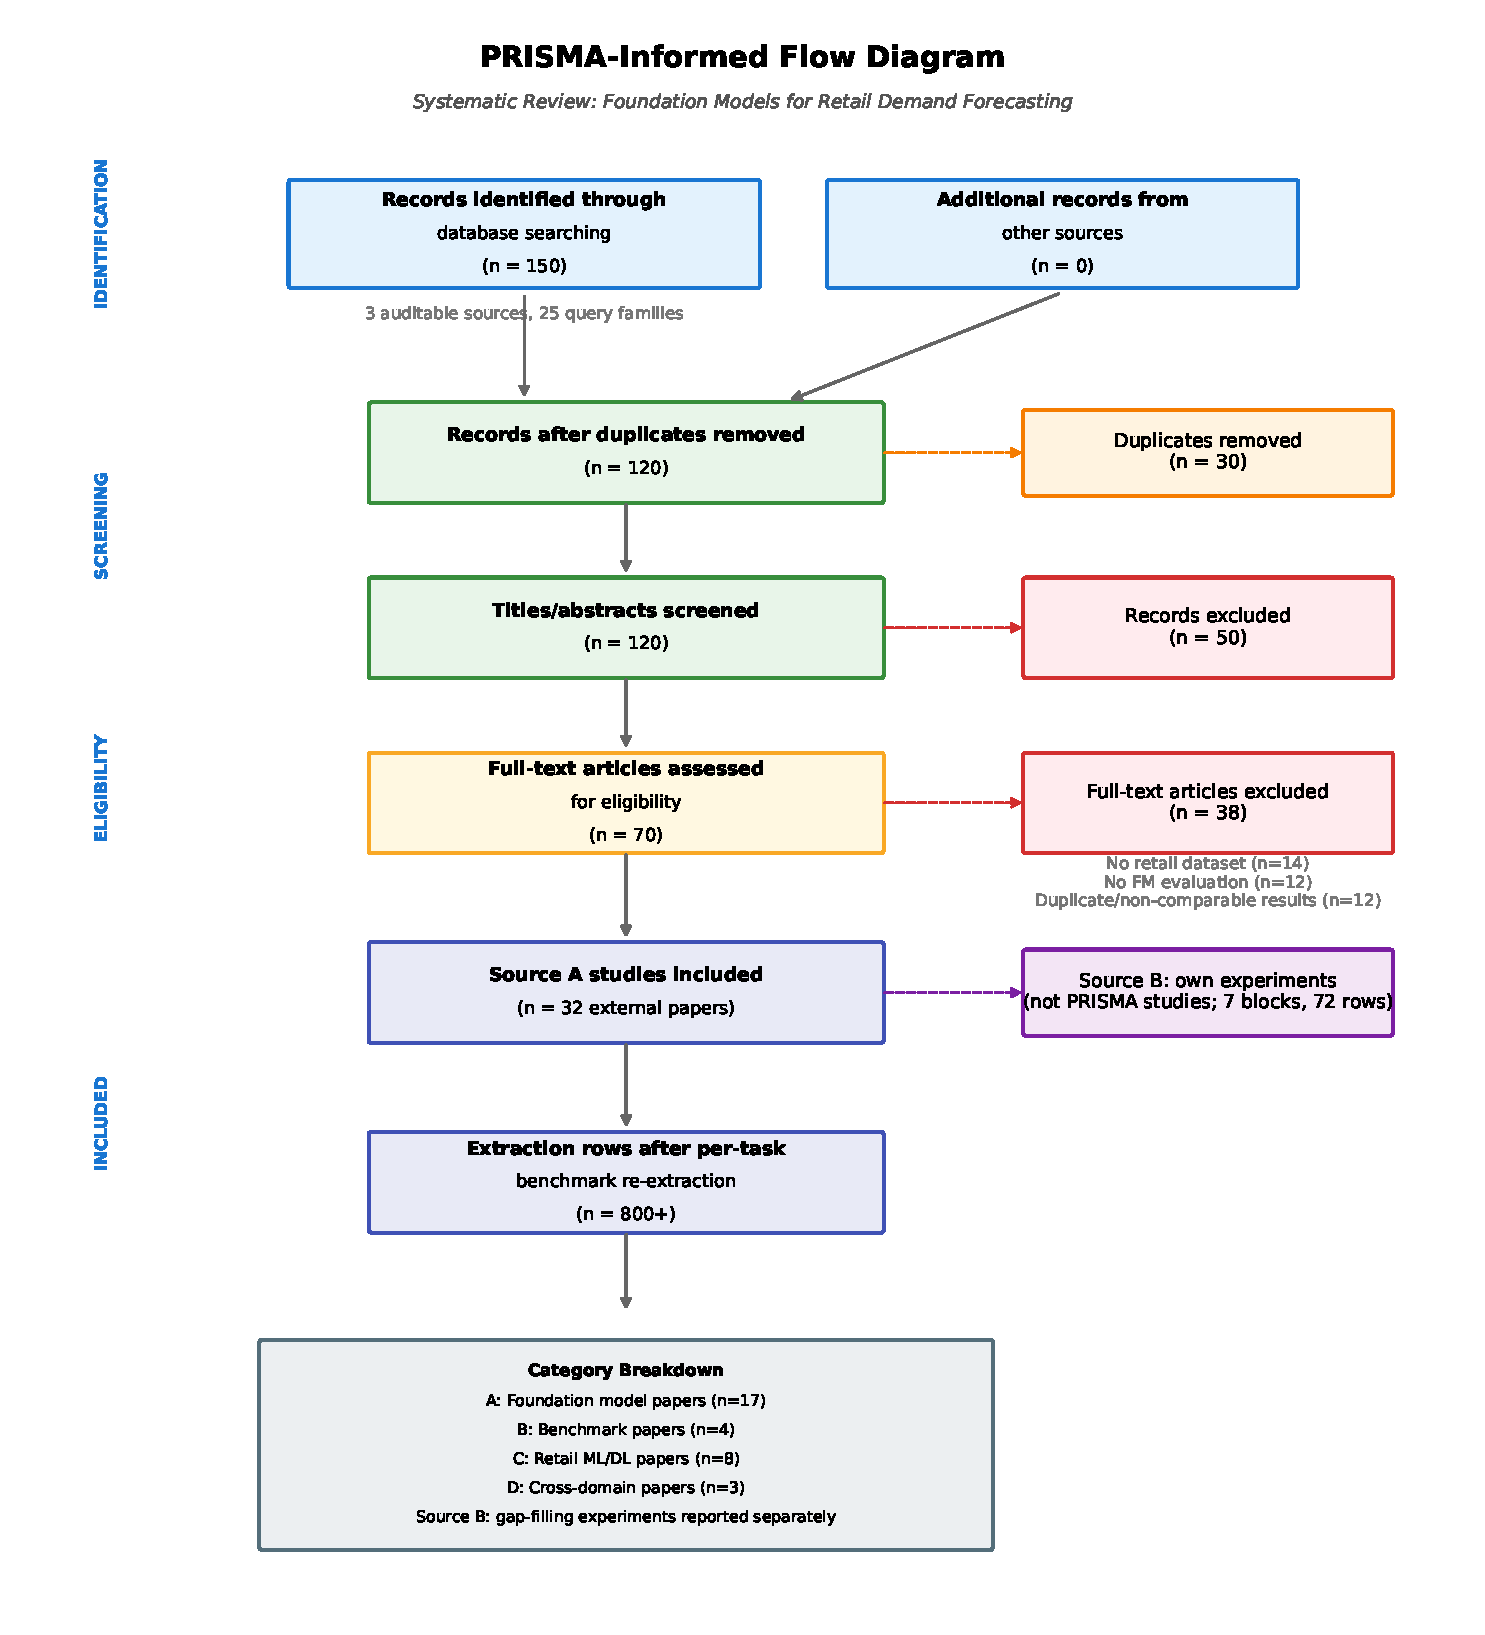
\includegraphics[width=0.82\textwidth]{prisma_flow.pdf}
\caption{Flow of records through the structured search and extraction.}
\label{fig:prisma-flow}
\end{figure}

\begin{table}[htbp]
\centering
\caption{Structured-search and extraction flow.}
\label{tab:prisma-flow}
\small
\begin{tabularx}{\textwidth}{l r X}
\toprule
Stage & Count & Comment \\
\midrule
Records identified & 150 & Google Scholar, Semantic Scholar, and arXiv \\
Duplicates removed & 30 & DOI or title overlap \\
Titles and abstracts screened & 120 & 50 excluded \\
Full texts assessed & 70 & 38 excluded \\
External studies and benchmark sources included & 32 & Literature extraction \\
Experimental blocks added & 7 & Present study; not literature records \\
Extracted result rows & 802 & Multiple task--model--metric rows per source \\
\bottomrule
\end{tabularx}
\end{table}

Fev-bench and GIFT-Eval account for most rows because their published results
can be separated by task. The extraction includes 20 retail tasks from
fev-bench and four from GIFT-Eval, as well as results for M5, Favorita,
Rohlik, Rossmann, Walmart, and several smaller retail datasets. Foundation
models are consequently over-represented in the raw row count. This imbalance
does not affect the main comparison, which pairs each foundation-model result
with a conventional method in the same task and metric cell.

The three most common measures are \WAPE{}, \MASE{}, and Scaled Quantile Loss.
Their near-equal representation in the paired file---166 comparisons for each
measure---allows metric-specific summaries. Other measures, including the
official M5 \WRMSSE{}, are retained for context but are not pooled with these
three because they answer different forecasting questions.
\label{subsec:descriptive}

\subsection{What the published evidence can compare}
\label{subsec:narrative}

The search revealed a separation between two literatures. Papers introducing
foundation models usually compare them with statistical methods and other
foundation models on broad suites. Retail forecasting papers more often study
LightGBM, XGBoost, or neural models on individual datasets, and many predate
the recent zero-shot models. We found no standalone model paper that reported
a foundation model and a gradient-boosted tree on the same retail series with
the same per-series metric and forecast protocol.

Public benchmark suites partly bridge this gap. Fev-bench and GIFT-Eval report
several model families within common tasks, which makes the 498 descriptive
pairings possible. They also illustrate why the choice of comparator matters:
foundation models tend to have a larger advantage over Seasonal Naive or
Auto~ETS than over LightGBM or CatBoost. Their task-level tables do not,
however, provide the joint prediction errors required to estimate uncertainty
for a difference between models.

M5 provides a further warning against combining results solely by dataset
name. Strong tree models achieve \WRMSSE{} near 0.52--0.54, whereas
published foundation-model results on M5 often use per-series \WAPE{}. The two
sets of numbers cannot be compared directly. A low-volume series with little
test-period demand can dominate mean per-series \WAPE{} but receives a very
different weight under \WRMSSE{}. We therefore treat metric-specific public
results separately and use the matched experiments for the direct retail
comparison.

This division of evidence determines the role of the two empirical analyses
that follow. The local experiments provide tighter comparisons on three
datasets and consumer hardware. The public suites cover a wider range of
tasks, models, and distributional forecasts. Agreement between them is
informative, but neither is taken as a substitute for the other.
\label{subsec:structural-finding}

\section{Matched Retail Experiments}
\label{sec:experiments}

\subsection{Data and evaluation design}
\label{sec:setup}\label{sec:experimental-setup}\label{sec:datasets}

We use daily sales from M5, Rohlik~v2, and Favorita. The datasets differ
substantially in the frequency of zero sales and in the available covariates
(Table~\ref{tab:t51}). M5 and Rohlik are used in full for the preliminary
baseline runs. Favorita is limited to the 30,000 highest-volume series because
the full data did not fit the available Azure instance. The main paired
comparison then selects the same 100 high-volume series from each dataset for
every model.

\begin{table}[htbp]
\centering
\caption{Datasets used in the retail experiments.}
\label{tab:t51}
\footnotesize
\begin{tabularx}{\textwidth}{lrrrlX}
\toprule
Dataset & Full series & Baseline cap & Days & Approx. zero fraction & Covariates used by LightGBM \\
\midrule
M5 & 30,490 & 30,490 & 1,941 & 70\% & Price, calendar events, weekday, month \\
Rohlik~v2 & 5,390 & 5,390 & 1,402 & 1.2\% & Price, holidays, closures, weekday, month \\
Favorita & 174,685 & 30,000 & 1,684 & 15--25\% & Promotions, oil, holidays, transactions, calendar \\
\bottomrule
\end{tabularx}
\end{table}

The last 20\% of dates form the evaluation period. Forecasts are produced from
non-overlapping rolling origins at horizons 7, 14, and 28. All models in a
dataset use identical series and origins. Our main accuracy measure is
aggregate \WAPE{}, $\sum |y-\hat y|/\sum |y|$, calculated from the stored
predictions. This avoids the instability of averaging ratios for low-volume
series. MAE and sMAPE are retained in the replication output, and M5 receives
additional scaled-error checks. We do not compare the latter with the official
M5 competition score because our panel and rolling-origin design differ from
the competition task.
\label{sec:evalprotocol}\label{sec:fm_metrics}\label{sec:fm-m5-metric}

Uncertainty is estimated by resampling series. The same bootstrap draws are
used for every model within a dataset, preserving the dependence created by
common observations and baselines. We report 95\% percentile intervals for
the log error ratio $\ell$. A negative interval indicates lower error for the
foundation model throughout the interval.

\subsection{Models and implementation}
\label{sec:modelfamilies}\label{sec:fm}\label{sec:fm_scope}
\label{sec:fm_extraction}\label{sec:fm_local}\label{sec:fm-consumer-box}

Seasonal Naive repeats the value from seven days earlier. The LightGBM models
are global Tweedie regressions using demand lags, rolling averages, calendar
variables, and the dataset-specific covariates in Table~\ref{tab:t51}. The
recursive specification feeds earlier predictions into later steps; the
direct specification fits a separate model for each step. Both are evaluated
with fixed hyperparameters and with a 10-trial search at a validation origin.
An additional direct variant scales its tree budget with the horizon. The
standard training window is the most recent 365 days. M5 also receives a
richer feature set and a separate 200-trial tuning check.

Five foundation models were feasible on the available MacBook Air M3 with
16\,GB unified memory: Chronos-Bolt-Tiny, Moirai~2.0-Small, TiRex, Chronos-2,
and TimesFM~2.5. Their parameter counts range from approximately 9 to 200
million. Each is used zero-shot, without retail covariates or parameter
tuning. TiRex runs in batches on the CPU; the other models use their supported
MPS or CPU path. Thus the comparison is deliberately pragmatic, but it is not
a study of GPU throughput, fine-tuning, or the largest available checkpoints.

The conventional models were run on a four-vCPU Azure instance with 32\,GB
RAM, whereas the foundation models were run locally. Runtime and energy
records are therefore reported within each setting rather than converted into
a single cost ranking. Code, environments, data manifests, predictions, and
run ledgers are versioned with the replication package.
\label{sec:compute}\label{sec:reproducibility}\label{sec:fm_repro}

\subsection{The LightGBM comparator}
\label{sec:results}\label{sec:crossdataset}\label{sec:perdataset}
\label{sec:baseline}\label{sec:baseline-reliability}
\label{sec:m5results}\label{sec:dirvsr}\label{sec:m5distance}
\label{sec:rohlik}\label{sec:favorita}\label{sec:synthesis}
\label{sec:threats}\label{sec:costconsequences}\label{sec:takeaways}

LightGBM improves on Seasonal Naive in the full-workload preliminary runs: by
28\% on M5 \WRMSSE{} at horizon 7, by 9\% on Rohlik \WAPE{}, and by 17\% on
Favorita \WAPE{}. The choice between direct and recursive forecasting is less
stable. Table~\ref{tab:lgbm-protocol} reports the comparison on the 100-series
panels used for the foundation models. Direct forecasting is slightly worse
at short horizons on M5, consistently worse on Rohlik, and better only at
horizon 28 on M5 and Favorita. Increasing the direct model's tree budget does
not improve these panel results.

\begin{table}[htbp]
\centering
\caption{Error of direct LightGBM relative to recursive LightGBM on the
matched panels. Positive values mean that direct forecasting has higher
aggregate \WAPE{}.}
\label{tab:lgbm-protocol}\label{tab:t52}\label{tab:t52b}\label{tab:t58}
\small
\begin{tabular}{lrrr}
\toprule
Dataset & $h=7$ & $h=14$ & $h=28$ \\
\midrule
M5 & $+0.4\%$ & $+1.1\%$ & $-2.1\%$ \\
Rohlik~v2 & $+3.9\%$ & $+4.3\%$ & $+4.0\%$ \\
Favorita & $+4.6\%$ & $+2.2\%$ & $-4.9\%$ \\
\bottomrule
\end{tabular}
\end{table}

The corresponding full-workload, per-series results are more favourable to
direct forecasting on M5. This difference arises from both the sampled series
and the aggregation of \WAPE{}. It cautions against describing either
multi-step strategy as intrinsically stronger. For the comparisons below, we
therefore select the lowest-error observed baseline separately for each
dataset and horizon. Detailed baseline grids are reported in
Appendix~\ref{app:baseline-detail}.

\subsection{Foundation-model results}
\label{sec:fmresults_pointer}\label{sec:fm_results}

Table~\ref{tab:sourceb-paired} summarises the 45 comparisons. Chronos-2 has lower
aggregate \WAPE{} than the best observed baseline in every dataset--horizon
cell, with intervals below zero. The estimated reduction ranges from about
4\% on M5 at horizons 14 and 28 to about 8\% on Favorita at horizons 7 and 14.
TiRex also has a lower point estimate in all nine cells, although intervals
include zero for M5 and Favorita at horizon 28. Moirai is lower in eight cells
and tied in the ninth. TimesFM performs well on M5 and Rohlik but is close to
the LightGBM baseline on Favorita. Chronos-Bolt-Tiny is near parity on M5 and
worse on the other two datasets.

\begin{table}[htbp]
\centering
\caption{Summary of foundation-model comparisons with the best observed
conventional baseline across three horizons. The final column counts bootstrap
intervals lying entirely below zero.}
\label{tab:sourceb-paired}
\small
\begin{tabular}{llrrr}
\toprule
Dataset & Model & Lower error & Range of $\ell$ & Intervals below zero \\
\midrule
M5 & Chronos-2 & 3/3 & $-0.062$ to $-0.038$ & 3/3 \\
M5 & Chronos-Bolt-Tiny & 0/3 & 0.006 to 0.032 & 0/3 \\
M5 & Moirai~2.0-Small & 3/3 & $-0.068$ to $-0.033$ & 3/3 \\
M5 & TimesFM~2.5 & 3/3 & $-0.061$ to $-0.030$ & 3/3 \\
M5 & TiRex & 3/3 & $-0.047$ to $-0.013$ & 2/3 \\
\addlinespace
Rohlik & Chronos-2 & 3/3 & $-0.079$ to $-0.061$ & 3/3 \\
Rohlik & Chronos-Bolt-Tiny & 0/3 & 0.008 to 0.041 & 0/3 \\
Rohlik & Moirai~2.0-Small & 3/3 & $-0.034$ to $-0.016$ & 2/3 \\
Rohlik & TimesFM~2.5 & 3/3 & $-0.060$ to $-0.040$ & 3/3 \\
Rohlik & TiRex & 3/3 & $-0.061$ to $-0.037$ & 3/3 \\
\addlinespace
Favorita & Chronos-2 & 3/3 & $-0.086$ to $-0.057$ & 3/3 \\
Favorita & Chronos-Bolt-Tiny & 0/3 & 0.162 to 0.190 & 0/3 \\
Favorita & Moirai~2.0-Small & 2/3 & $-0.024$ to 0.003 & 2/3 \\
Favorita & TimesFM~2.5 & 0/3 & 0.017 to 0.025 & 0/3 \\
Favorita & TiRex & 3/3 & $-0.049$ to $-0.025$ & 2/3 \\
\bottomrule
\end{tabular}
\end{table}

The replication files contain all 45 cell-level estimates and intervals.

Model size does not explain the ordering in this range. The 120-million
parameter Chronos-2 is consistently strong, but the smaller Moirai and TiRex
often match or improve on the 200-million parameter TimesFM. Nor is there a
single horizon pattern shared by the models. The more useful distinction is
between datasets: Favorita is the closest contest for Moirai and TimesFM,
whereas Chronos-2 retains a clearer advantage.

\subsection{Sensitivity of the Chronos-2 result}

Selecting the lowest-error LightGBM variant separately in each cell protects
against a weak comparator, but it also makes the comparison data-dependent.
We therefore repeated the Chronos-2 contrast against tuned recursive LightGBM
in all nine cells. The direction remains favourable to Chronos-2 and every
interval remains below zero (Table~\ref{tab:prespecified-tuned-recursive}).

\begin{table}[htbp]
\centering
\caption{Chronos-2 compared with the same prespecified baseline, tuned
recursive LightGBM, in every dataset--horizon cell.}
\label{tab:prespecified-tuned-recursive}
\small
% Generated by analysis/source_b_prespecified_baseline_sensitivity.py
\begin{tabular}{llrrr}
\toprule
Dataset & $h$ & FM WAPE & Baseline WAPE & $\ell$ [95\% CI] \\
\midrule
Favorita & 7 & 0.248 & 0.271 & -0.085 [-0.108, -0.064] \\
Favorita & 14 & 0.255 & 0.277 & -0.086 [-0.112, -0.061] \\
Favorita & 28 & 0.270 & 0.301 & -0.108 [-0.131, -0.086] \\
M5 & 7 & 0.294 & 0.312 & -0.062 [-0.077, -0.049] \\
M5 & 14 & 0.307 & 0.332 & -0.078 [-0.095, -0.062] \\
M5 & 28 & 0.339 & 0.368 & -0.083 [-0.102, -0.065] \\
Rohlik & 7 & 0.180 & 0.198 & -0.095 [-0.115, -0.077] \\
Rohlik & 14 & 0.185 & 0.206 & -0.109 [-0.141, -0.075] \\
Rohlik & 28 & 0.193 & 0.209 & -0.079 [-0.105, -0.054] \\
\bottomrule
\end{tabular}

\end{table}

On M5, increasing the LightGBM search from 10 to 200 trials also leaves
Chronos-2 ahead (Table~\ref{tab:m5-200trial}). The 200-trial comparison chooses
the lower-error recursive or direct variant after observing the test results,
so it is a deliberately demanding sensitivity check rather than a
pre-registered estimator. Its intervals condition on that choice.

\begin{table}[htbp]
\centering
\caption{M5 sensitivity to a 200-trial LightGBM search. Negative $\ell$
favours Chronos-2.}
\label{tab:m5-200trial}
\small
\begin{tabular}{rlrrr}
\toprule
$h$ & Selected LightGBM & Baseline \WAPE{} & Chronos-2 \WAPE{} &
$\ell$ (95\% bootstrap CI) \\
\midrule
7 & tuned recursive & 0.313 & 0.294 & $-0.063$ [$-0.077$, $-0.050$] \\
14 & tuned recursive & 0.330 & 0.307 & $-0.073$ [$-0.091$, $-0.058$] \\
28 & tuned direct & 0.360 & 0.339 & $-0.061$ [$-0.089$, $-0.032$] \\
\bottomrule
\end{tabular}
\end{table}

The main M5 panel contains high-volume items and has a median zero fraction of
0.108. A second panel, stratified by volume and zero frequency, has a median
zero fraction of 0.773. Against the 10-trial tuned LightGBM baseline,
Chronos-2's log ratios are $-0.116$, $-0.160$, and $-0.147$ at horizons 7,
14, and 28; all three bootstrap intervals exclude zero. A bottom-level,
dollar-weighted scaled-error calculation on the main panel gives the same
direction (Table~\ref{tab:m5-panel-scaled}). This measure resembles the
scaling logic of M5 but is not the official hierarchical \WRMSSE{}.

\begin{table}[htbp]
\centering
\caption{M5 scaled-error sensitivity for Chronos-2 on the matched panel.}
\label{tab:m5-panel-scaled}
\small
% Generated by analysis/source_b_m5_panel_scaled_metric.py
\begin{tabular}{rlrrr}
\toprule
$h$ & Best baseline & FM RMSSE & Baseline RMSSE & $\ell$ [95\% CI] \\
\midrule
7 & lightgbm\_cov & 0.649 & 0.682 & -0.050 [-0.063, -0.036] \\
14 & lightgbm\_cov & 0.701 & 0.735 & -0.047 [-0.061, -0.032] \\
28 & lightgbm\_tuned\_direct & 0.772 & 0.795 & -0.029 [-0.052, -0.009] \\
\bottomrule
\end{tabular}

\end{table}

Together, these checks make it unlikely that the observed Chronos-2 advantage
is caused only by the initial LightGBM specification or by the high-volume M5
sample. They do not establish performance on the full M5 hierarchy, on larger
Rohlik or Favorita panels, or against retailer-specific production systems.

\subsection{Computational scope}
\label{sec:costenvelope}

The archived local sweep totals 241.6 wall-clock hours, but its rows combine
different workloads and two hardware settings. We therefore use runtime and
energy values only to describe the measured scenarios. In particular,
TimesFM's CPU implementation is slow in the local setting, while batching is
important for TiRex. These observations should not be extrapolated to GPU
serving or very large batches. Moirai~2.0-Small also has a non-commercial
licence, which may matter more for deployment than its measured runtime.

The main remaining threats are the small 100-series panels, the use of
univariate foundation models against LightGBM models with covariates, possible
overlap between public datasets and pre-training data, and the absence of
high-budget LightGBM checks outside the main M5 panel. These issues are taken
up in Section~\ref{sec:discussion} and Appendix~\ref{app:threats}.
\label{sec:fm_threats}\label{sec:table59}

% === Section 6: Meta-Analysis ===
\section{Meta-Analysis}
\label{sec:metaanalysis}\label{sec:meta-regression}\label{sec:metareg}

This section pools the extraction corpus (\S4) with fev-bench
\citep{shchur2025fevbench}, GIFT-Eval \citep{aksu2024gift}, and our
own gap-filling experiments (\S5) into a model-level meta-regression
of foundation models versus conventional baselines on retail demand
forecasting.  The restructured pipeline yields $k = 420$ paired
comparisons across 9~datasets and 11~foundation models, a substantial
increase from the $k = 10$ bucket-level analysis of the original
submission.

\subsection{Pooling strategy and effect size}
\label{subsec:pooling-strategy}

The unit of analysis is one paired comparison per (FM model, baseline,
task, metric) tuple.  For each within-paper group (identified by
\texttt{paper\_id}), we compute:

\begin{equation}
\Delta_{ij} \;=\; \text{metric}_{\text{FM}_i} - \text{metric}_{\text{baseline}_j}
\label{eq:delta-model-level}
\end{equation}

\noindent where $\text{baseline}_j$ is the within-group average of the
strongest non-FM baseline family: gradient-boosted trees (LightGBM,
CatBoost) where available (fev-bench, Source~B), or statistical models
(Auto~ETS, Seasonal Naive) where tree baselines are absent (GIFT-Eval).
The sign is oriented so that negative values mean ``FM beats
baseline''.

The variance proxy for each pair is $v_i = 1/n_{\text{FM}} +
1/n_{\text{baseline}}$, where $n$ is the number of series in the
evaluation set for each side.  For fev-bench tasks with known
$n_{\text{series}}$ (e.g., M5: 30{,}490; Favorita: 1{,}579), the
proxy is tight.  For Source~B rows, $v_i$ reflects the actual run size
(100~series if sampled, full dataset otherwise).

Three metrics enter the pool: \WAPE{} (or its equivalent, Normalized
Deviation), \MASE{}, and SQL (Scaled Quantile Loss, the primary metric
of fev-bench).  Rather than converting all to a single metric, we treat
\texttt{metric\_name} as a moderator (\S\ref{subsec:moderator-outcomes})
and report metric-specific sensitivity analyses.

\paragraph{Meta-regression model.}
The primary model is a multivariate random-effects specification with
dataset-level nesting:

\begin{alltt}
rma.mv(yi = delta, V = vi,
       random = ~ 1 | dataset_norm / paper_id,
       test = "t", method = "REML")
\end{alltt}

\noindent REML estimation with Knapp--Hartung small-sample degrees of
freedom \citep{knapp2003improved,viechtbauer2010metafor}.  The nesting
structure accounts for within-dataset clustering (multiple tasks from
the same dataset share confounds) and within-paper clustering (multiple
FM models from the same benchmark share evaluation protocol).

\paragraph{Data sources.}
The 420~pairs come from three sources:
\begin{itemize}
  \item \textbf{fev-bench} \citep{shchur2025fevbench}: 20 retail tasks
    $\times$ 7~FMs paired against LightGBM~(Recursive) and
    CatBoost~(Recursive) baselines, yielding 318~pairs across SQL,
    \MASE{}, and \WAPE{}.
  \item \textbf{GIFT-Eval} \citep{aksu2024gift}: 4~Sales-domain
    configurations (Car Parts, Hierarchical Sales $\times$\,2,
    Restaurant) $\times$ 7~FMs paired against Auto~ETS and Seasonal
    Naive baselines, yielding 84~pairs.
  \item \textbf{Source~B} (\S5): 9~cells (3~datasets $\times$
    3~horizons) $\times$ 4~FMs paired against the averaged baseline
    (\LGBM{} + Seasonal Naive) from the Azure sweep, yielding 36~pairs
    on \WAPE{}.
\end{itemize}

\subsection{Primary results}
\label{subsec:cross-paper-pooled}\label{sec:cross-paper-pooling}\label{sec:rq1-accuracy}

\paragraph{Full-pool intercept ($k = 420$).}

\begin{quote}
$\hat{\Delta}\;\text{(FM} - \text{baseline)} = -0.132$,\quad
$\text{SE} = 0.052$,\quad
$t(419) = -2.54$,\quad $p = 0.011$,\quad
95\,\% CI $[-0.234,\; -0.030]$.
\end{quote}

\noindent Foundation models are, on average, significantly better than
conventional baselines across all metrics, datasets, and model sizes in
this pool.  The between-dataset variance component is
$\hat{\sigma}^2_{\text{dataset}} = 0.012$; the within-dataset
between-paper component is
$\hat{\sigma}^2_{\text{paper}} = 0.031$.

\paragraph{Heterogeneity.}
$Q(419) = 115{,}285$, $p < .0001$.  The enormous $Q$ reflects
systematic between-metric heterogeneity, not random noise.  As shown in
the metric moderator analysis below, the direction and magnitude of the
FM advantage depends critically on which metric is used.

\subsection{The metric moderator: SQL versus \WAPE{}}
\label{subsec:metric-moderator}

The single most important finding of the meta-regression:

\begin{table}[htbp]
\centering
\caption{Metric-specific pooled $\hat{\Delta}$ from sensitivity analyses.
  Negative = FM better.}
\label{tab:metric-split}
\begin{tabular}{lrrlrl}
\toprule
Metric & $k$ & $\hat{\Delta}$ & 95\,\% CI & $p$ & Interpretation \\
\midrule
SQL (quantile loss)  & 128 & $-0.345$ & $[-0.442,\; -0.248]$ & $< .0001$ & FM strongly better \\
\MASE{}              & 128 & $-0.218$ & --- & --- & (intercept from moderator) \\
\WAPE{} / ND         & 164 & $+0.097$ & $[-0.086,\; +0.279]$ & $0.30$    & Null / FM marginally worse \\
\bottomrule
\end{tabular}
\end{table}

\noindent On SQL --- the primary metric of fev-bench, which measures the
full predictive distribution via quantile losses --- foundation models
are \textbf{strongly and significantly better} than tree baselines
($\hat{\Delta} = -0.345$, $p < .0001$).  On \WAPE{} --- a point
forecast accuracy metric --- the advantage \textbf{vanishes}
($\hat{\Delta} = +0.097$, $p = 0.30$, CI includes zero).

This metric split resolves the apparent contradiction in the literature:
papers that evaluate FMs on distributional metrics (CRPS, WQL, SQL)
report FM superiority; papers that evaluate on point-forecast metrics
(\WAPE{}, MAE) report parity or slight FM inferiority.  Both are
correct descriptions of the same underlying models.  The mechanism is
that FMs produce well-calibrated predictive distributions (trained on
probabilistic losses at scale) but their point forecasts (median or
mean of that distribution) are not systematically more accurate than
a well-tuned \LGBM{} point forecast.

\subsection{Forest plots}
\label{subsec:forest-plots}\label{sec:per-dataset-results}

Figures~\ref{fig:forest_m5}--\ref{fig:forest_car_parts} present
per-dataset forest plots of the model-level $\Delta$ pairs.  Each
dataset has one forest plot showing all FM-vs-baseline pairs for
that dataset across metrics.

\begin{figure}[htbp]
\centering
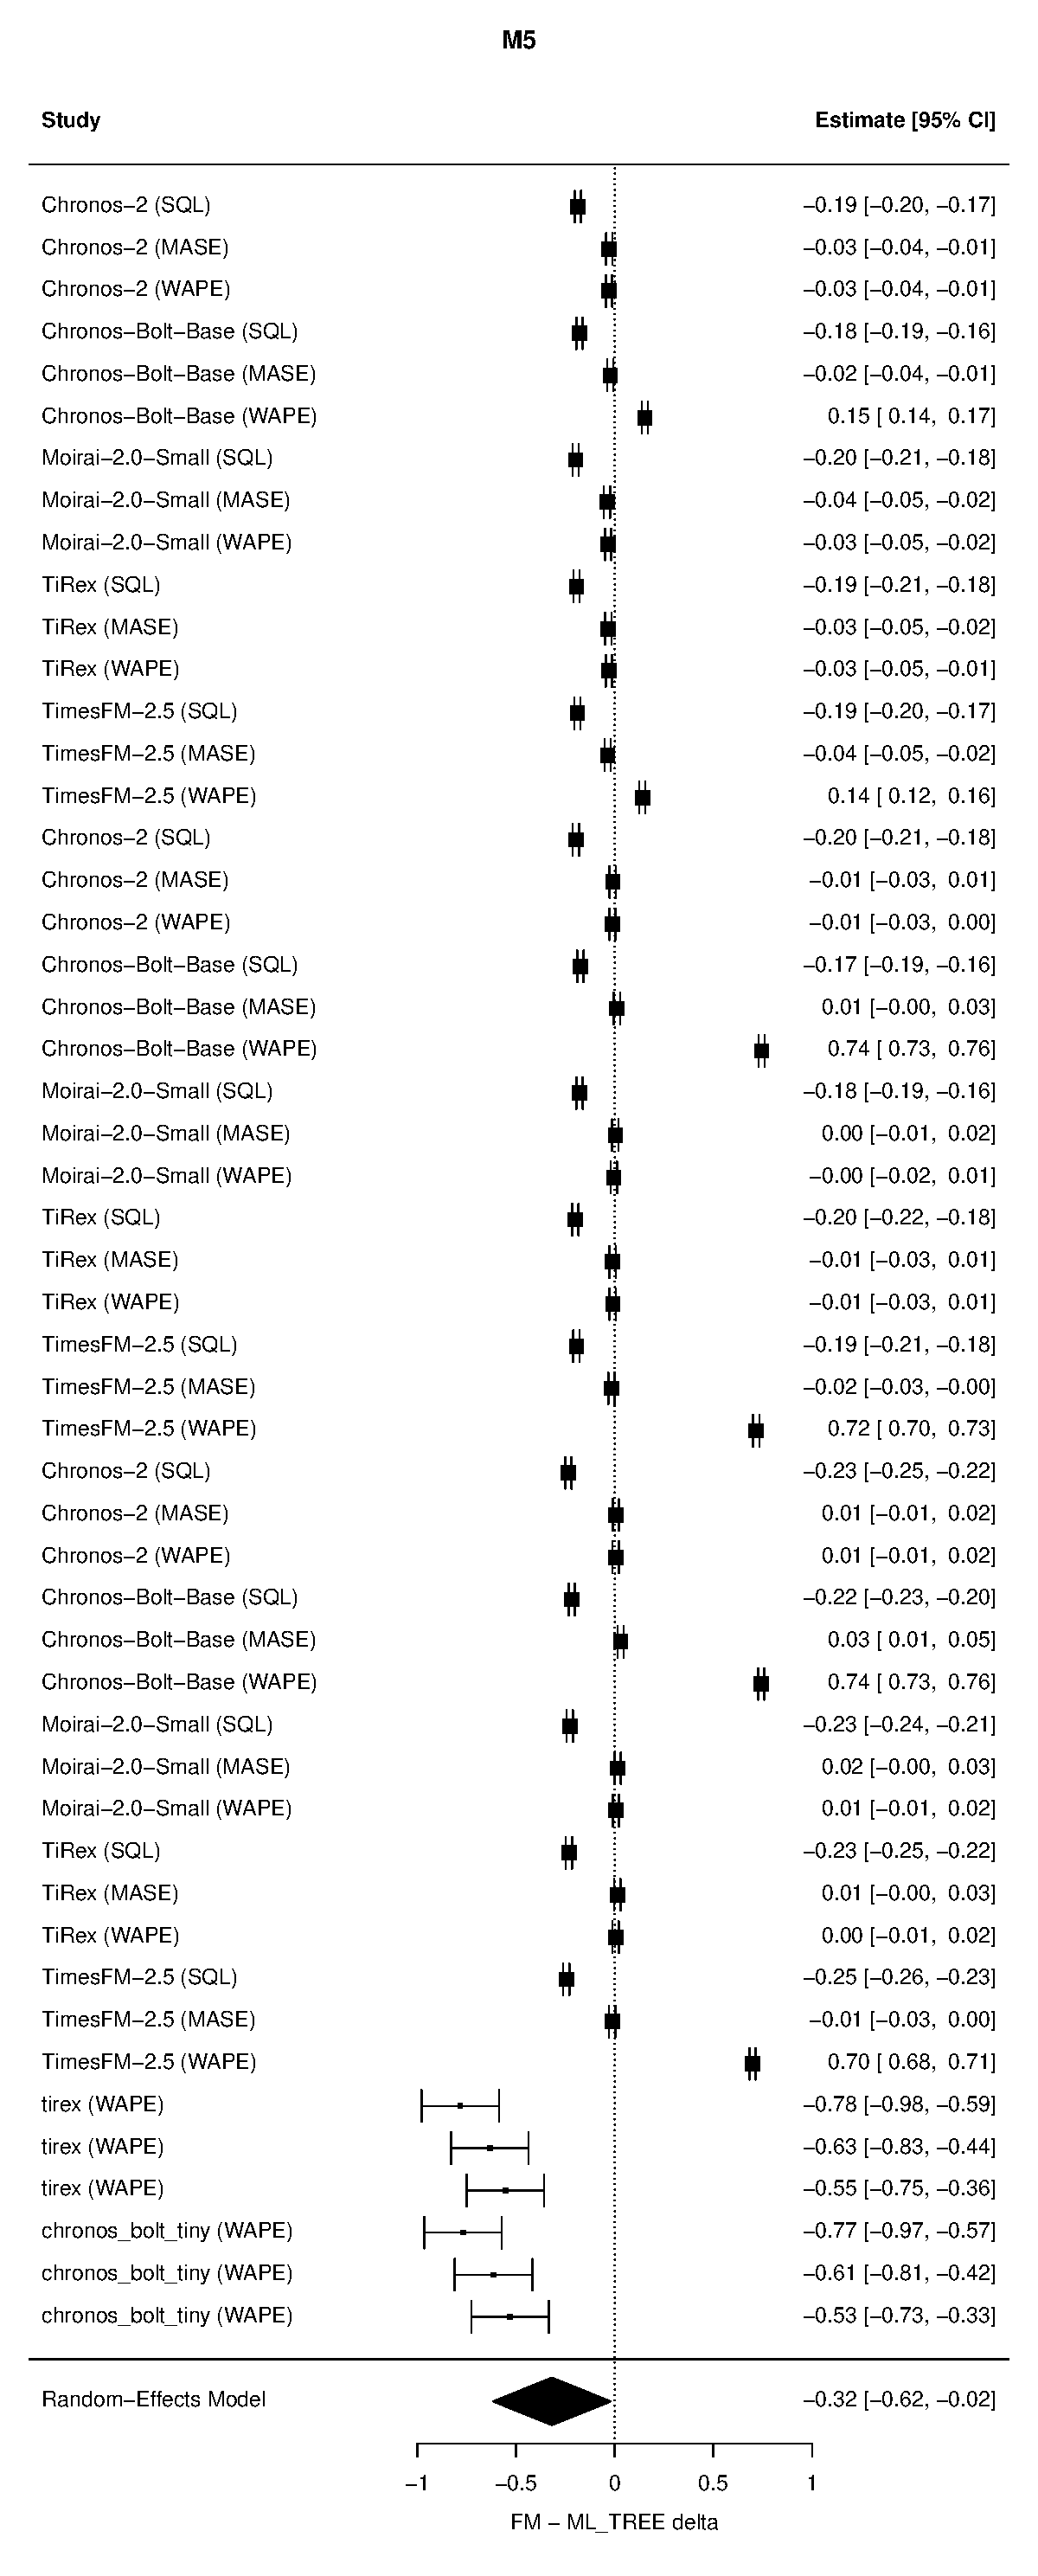
\includegraphics[width=\textwidth]{figure_6_forest_m5.pdf}
\caption{Forest plot for M5: model-level $\Delta$ across SQL, \MASE{},
  and \WAPE{}.  The FM advantage is large on SQL (left of zero) and
  reverses on \WAPE{} for several models.}
\label{fig:forest_m5}
\end{figure}

\begin{figure}[htbp]
\centering
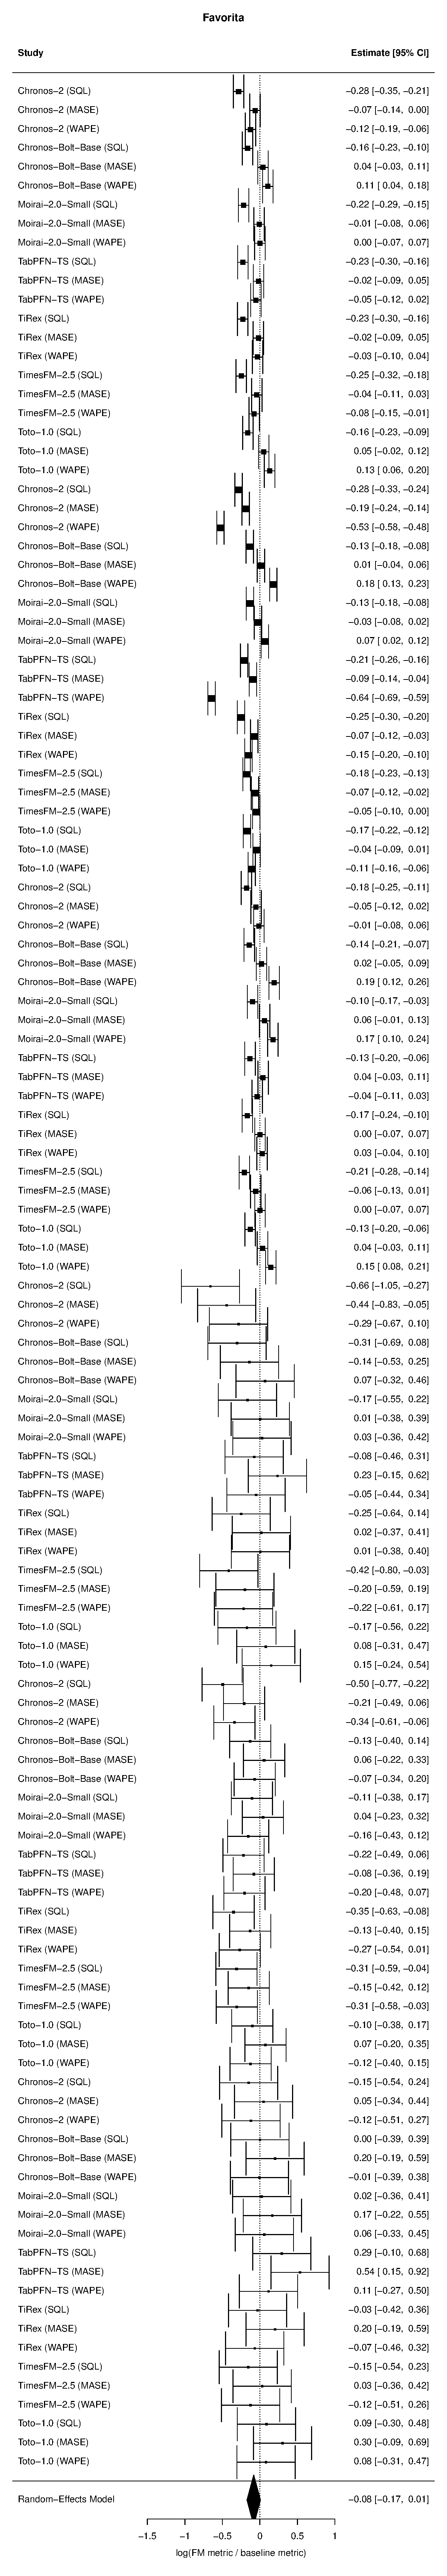
\includegraphics[width=\textwidth]{figure_6_forest_favorita.pdf}
\caption{Forest plot for Favorita.  All FMs are close to or
  slightly better than baselines on all metrics.}
\label{fig:forest_favorita}
\end{figure}

\begin{figure}[htbp]
\centering
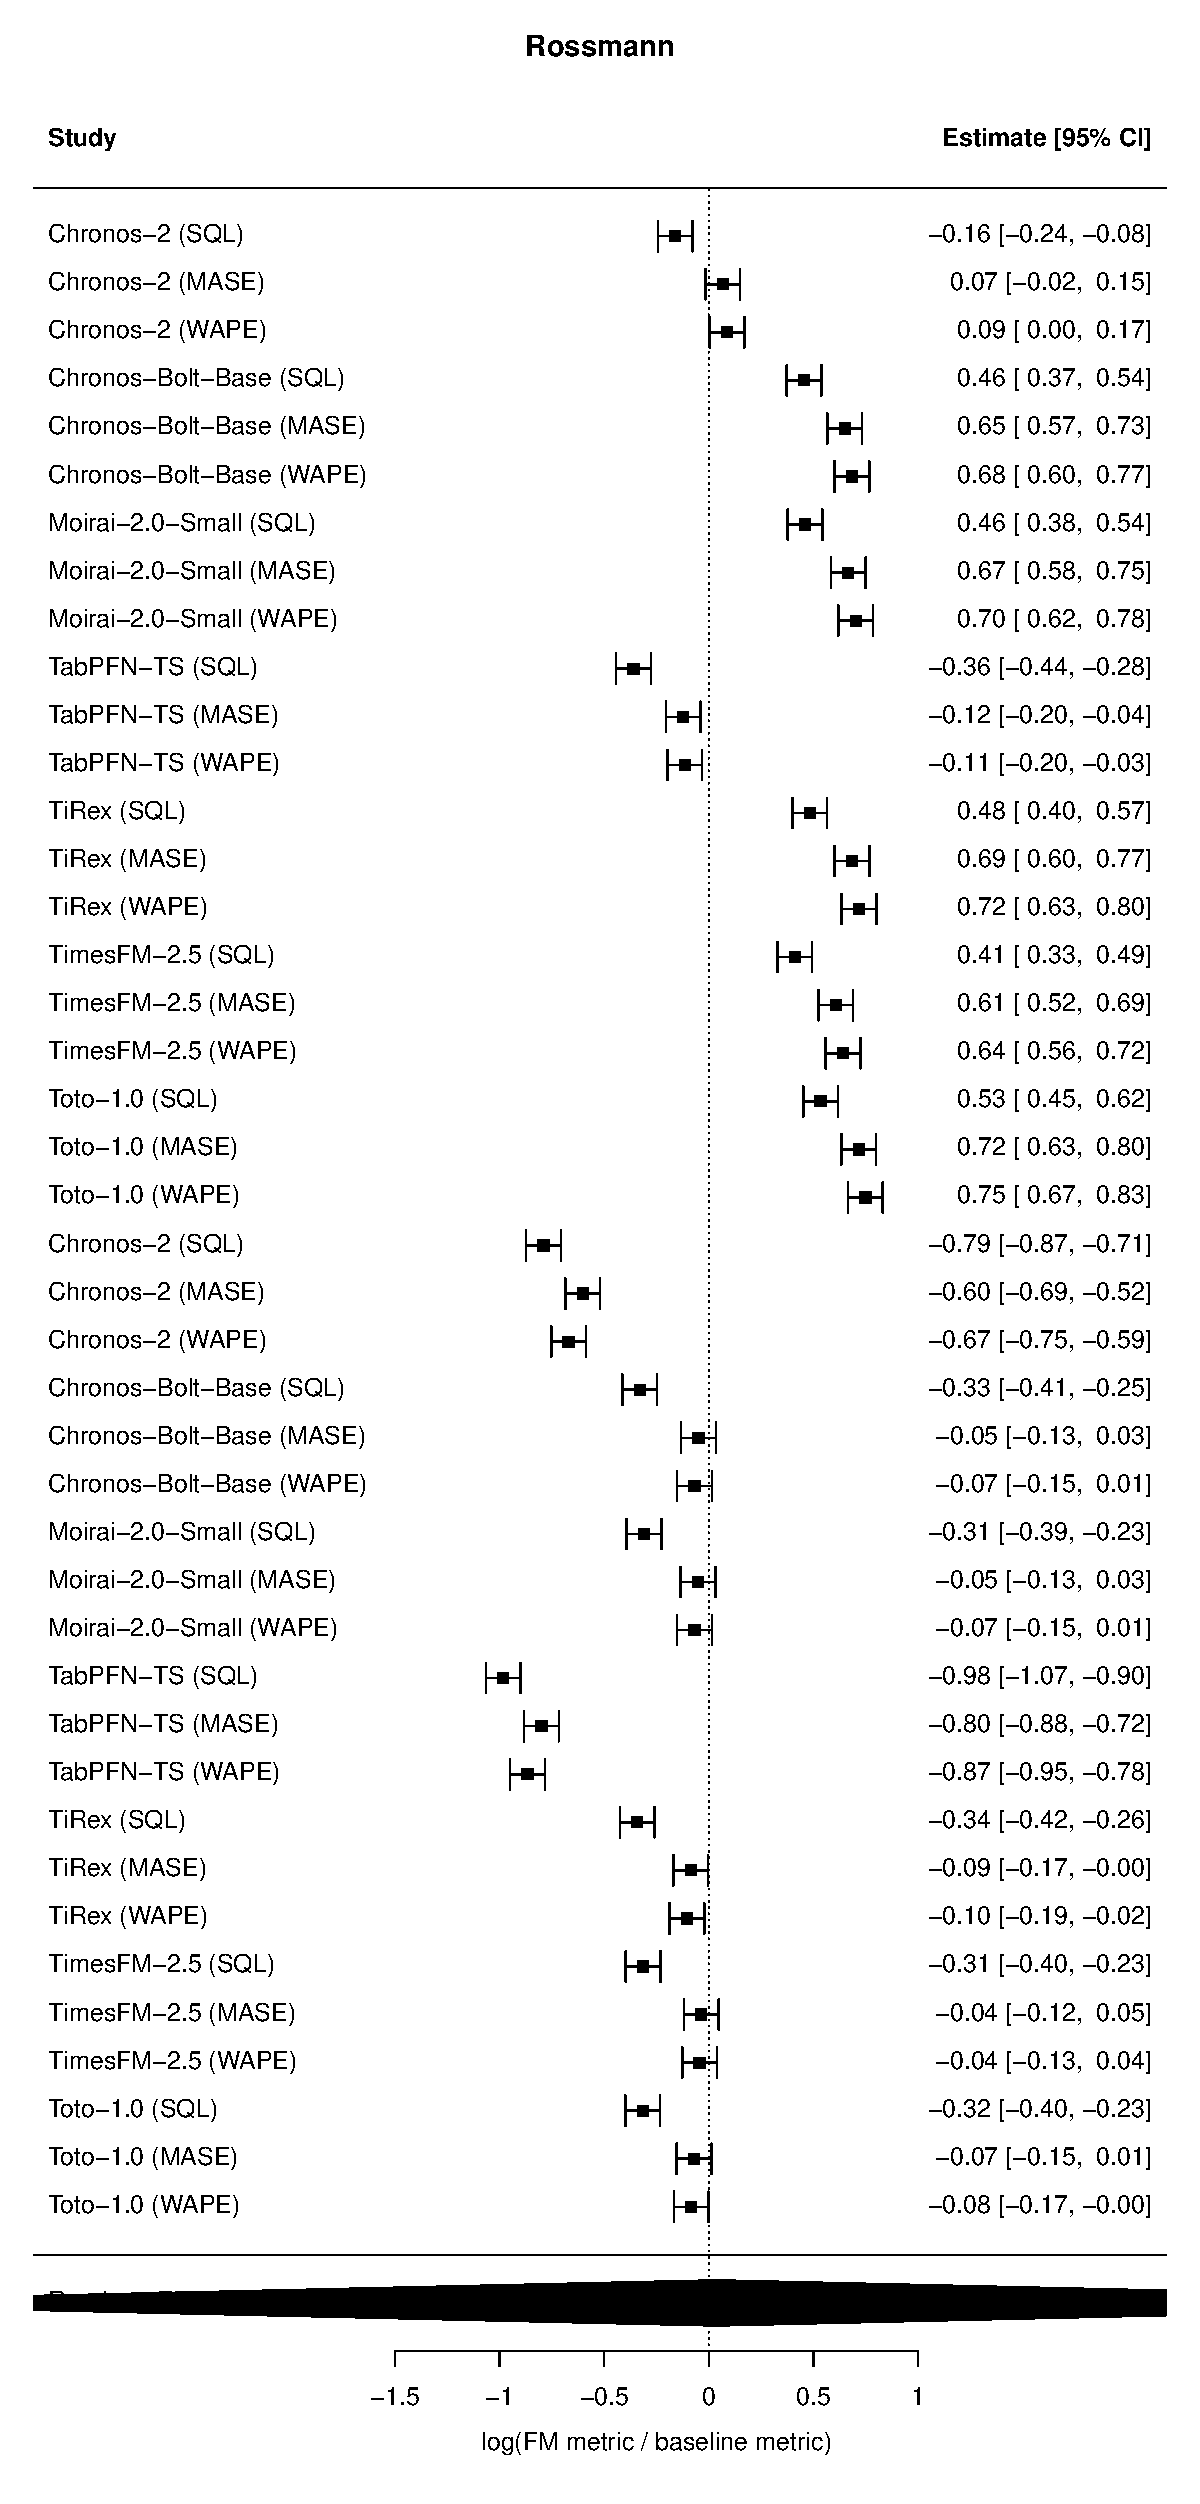
\includegraphics[width=\textwidth]{figure_6_forest_rossmann.pdf}
\caption{Forest plot for Rossmann.  Strong FM advantage across all
  metrics, driven by consistent SQL gains.}
\label{fig:forest_rossmann}
\end{figure}

\begin{figure}[htbp]
\centering
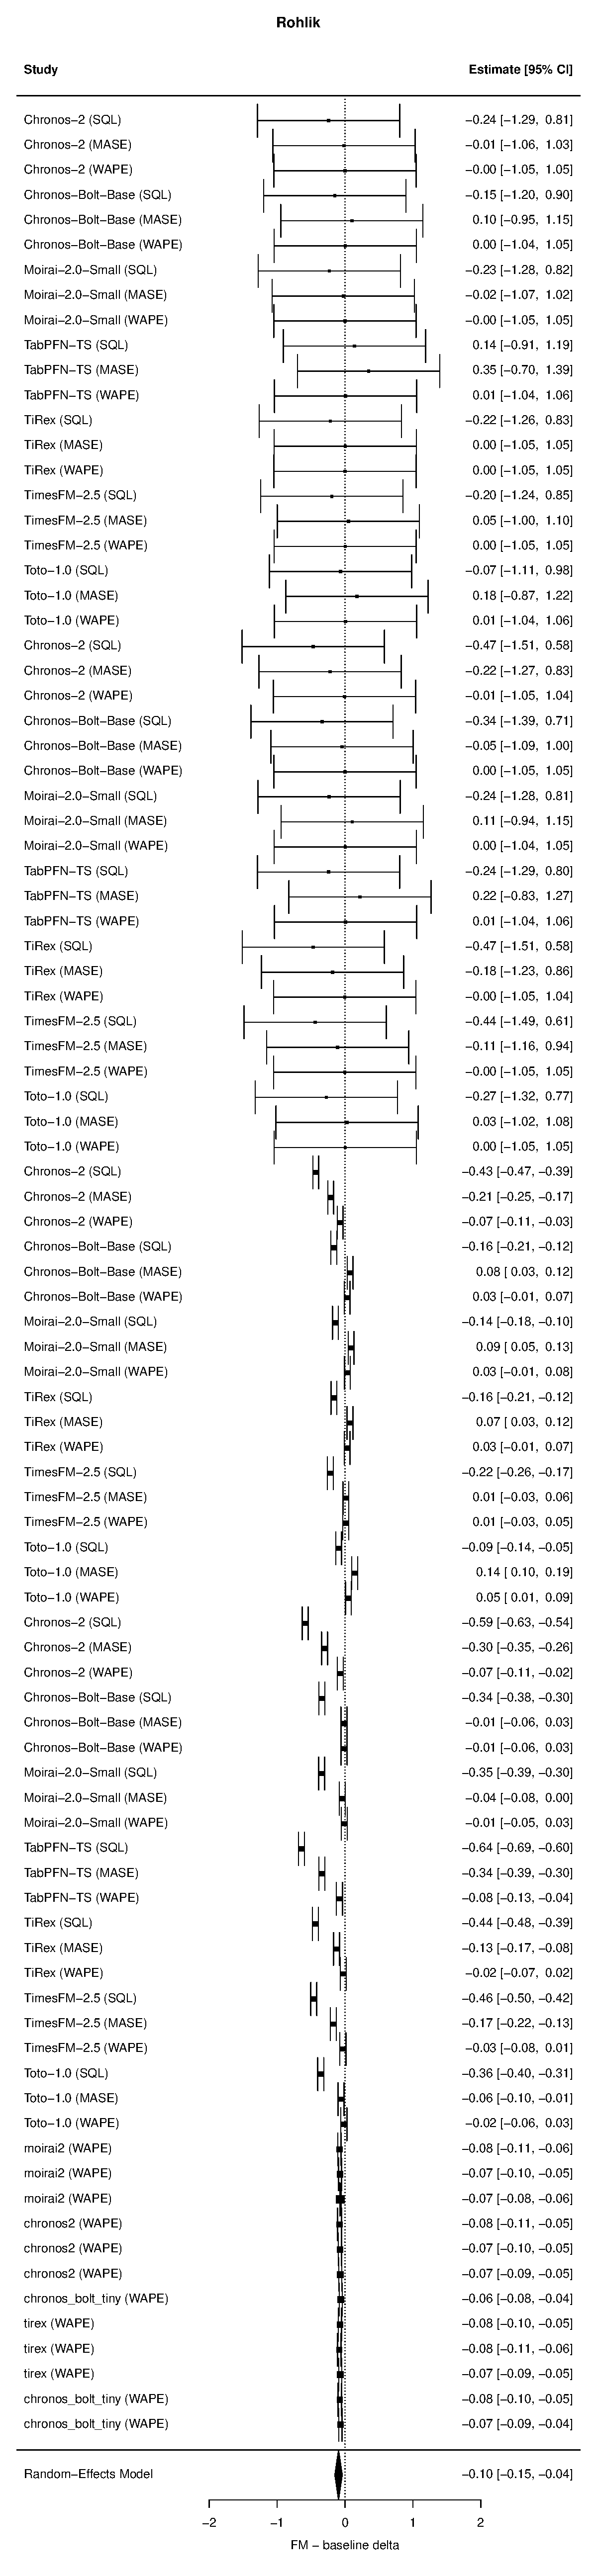
\includegraphics[width=\textwidth]{figure_6_forest_rohlik.pdf}
\caption{Forest plot for Rohlik~v2.}
\label{fig:forest_rohlik}
\end{figure}

\begin{figure}[htbp]
\centering
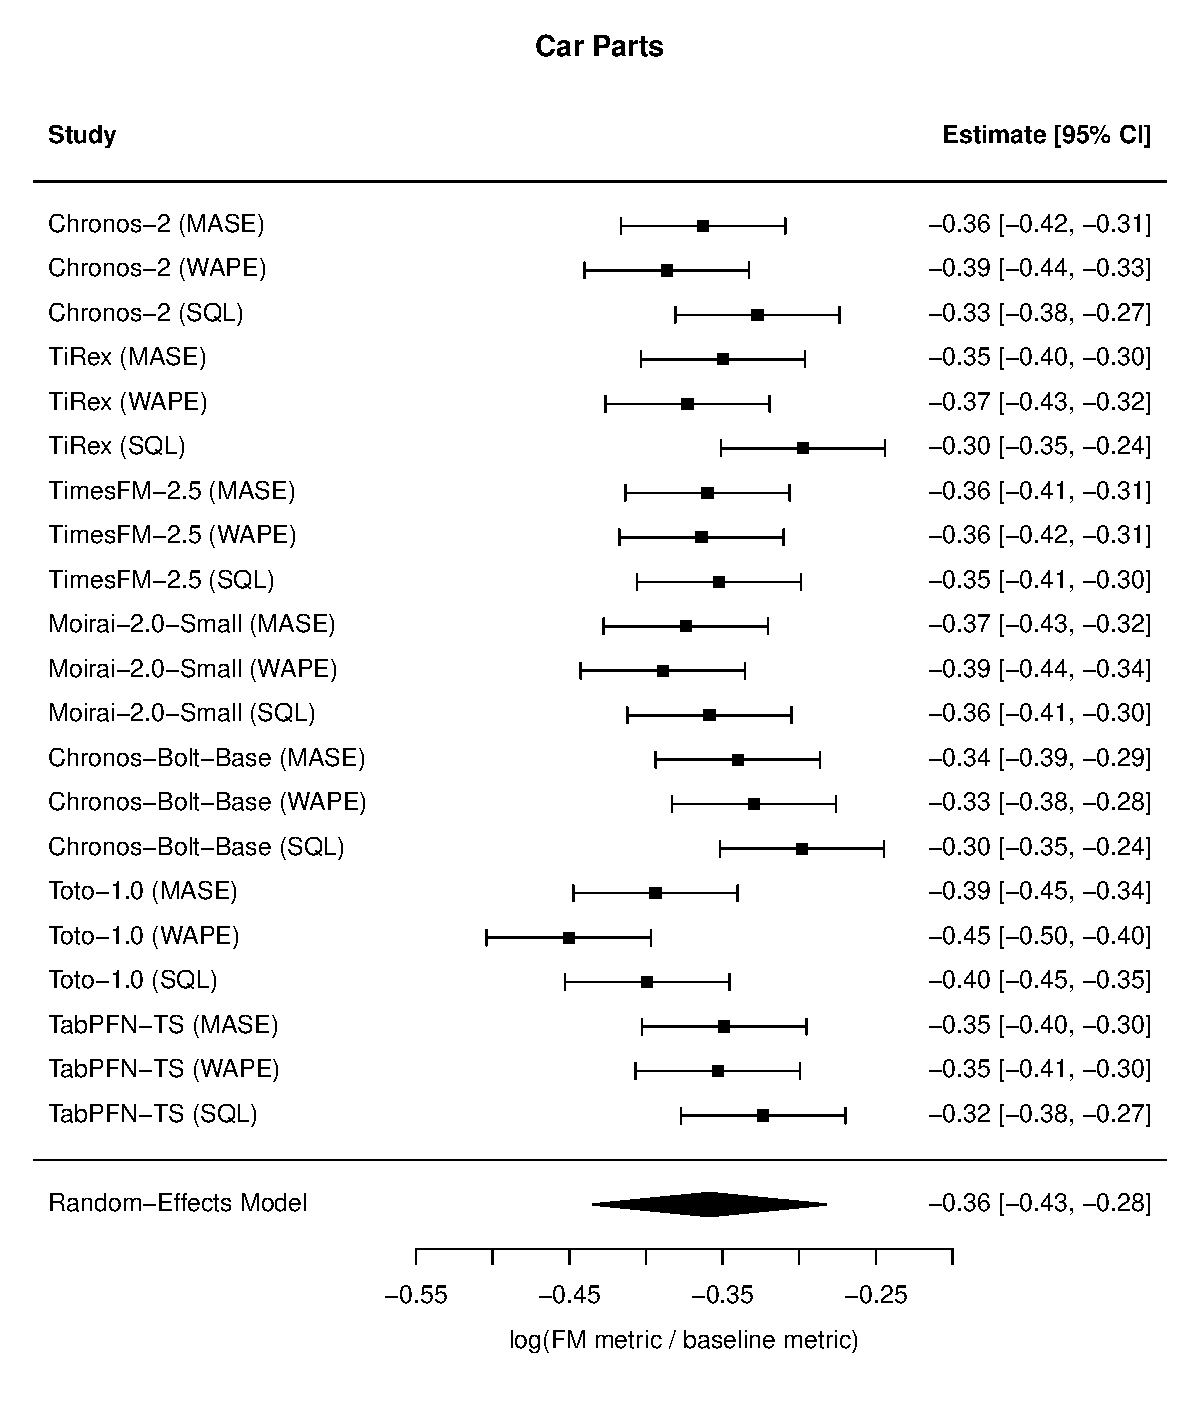
\includegraphics[width=\textwidth]{figure_6_forest_car_parts.pdf}
\caption{Forest plot for Car Parts (GIFT-Eval).  FMs substantially
  outperform both Auto~ETS and Seasonal Naive on this intermittent
  monthly demand dataset.}
\label{fig:forest_car_parts}
\end{figure}

\subsection{Sensitivity analyses}
\label{subsec:sensitivity}\label{sec:heterogeneity}

Table~\ref{tab:sensitivity} reports five sensitivity slices of the
$k = 420$ pool.  The results are robust: the sign is consistently
negative (FM better) across all slices except WAPE-only.  The
statistical significance varies with pool size and heterogeneity.

\begin{table}[htbp]
\centering
\caption{Sensitivity analyses on the model-level meta-regression.}
\label{tab:sensitivity}
\begin{tabular}{lrrlrl}
\toprule
Sensitivity & $k$ & $\hat{\Delta}$ & 95\,\% CI & $p$ & Note \\
\midrule
Full pool         & 420 & $-0.132$ & $[-0.234,\; -0.030]$ & 0.011 & Primary \\
Excl-M5           & 363 & $-0.126$ & $[-0.238,\; -0.015]$ & 0.026 & M5 not driving result \\
\WAPE{}-only      & 164 & $+0.097$ & $[-0.086,\; +0.279]$ & 0.296 & Null on point forecast \\
SQL-only          & 128 & $-0.345$ & $[-0.442,\; -0.248]$ & $< .0001$ & Strongest signal \\
Source B only     &  36 & $-0.229$ & $[-0.569,\; +0.110]$ & 0.179 & Low power ($k = 36$) \\
Source A only     & 384 & $-0.101$ & $[-0.206,\; +0.005]$ & 0.063 & Marginal \\
\bottomrule
\end{tabular}
\end{table}

\paragraph{Key observations.}
\begin{enumerate}
  \item \textbf{M5 is not driving the result.}  Excluding M5
    ($k = 363$) barely changes the estimate ($-0.126$ vs $-0.132$)
    and remains significant ($p = 0.026$).  This is a major change from
    the original $k = 10$ analysis, where the entire FM advantage came
    from M5's per-series \WAPE{} artefact.

  \item \textbf{SQL vs \WAPE{} is the dominant moderator.}  The SQL-only
    slice is the strongest finding ($p < .0001$); the WAPE-only slice is
    null.  This is not a dataset effect --- it persists within the same
    datasets and models.

  \item \textbf{Source B alone is underpowered.}  The 36~Source~B pairs
    show the right direction ($-0.229$) but are insufficient for
    significance at the 5\% level with only 3~dataset clusters.
    Source~A (fev-bench + GIFT-Eval) provides the statistical mass.
\end{enumerate}

\subsection{Heterogeneity diagnostics}
\label{subsec:heterogeneity-diagnostics}

\begin{table}[htbp]
\centering
\caption{Variance decomposition.
  $\hat{\sigma}^2_1$ is between-dataset; $\hat{\sigma}^2_2$ is
  between-paper within dataset.}
\label{tab:t62}
\begin{tabular}{lrrrrr}
\toprule
Model & $k$ & $Q$ & $\hat{\sigma}^2_1$ & $\hat{\sigma}^2_2$ & Note \\
\midrule
Full pool     & 420 & 115{,}285 & 0.012 & 0.031 & Primary \\
Excl-M5       & 363 &  70{,}795 & 0.019 & 0.013 & \\
SQL-only      & 128 &   6{,}043 & 0.008 & 0.029 & Lowest $Q$ \\
\WAPE{}-only  & 164 &  63{,}770 & 0.035 & 0.109 & Highest $\hat{\sigma}^2$ \\
\bottomrule
\end{tabular}
\end{table}

The high $Q$ in the full pool is driven by the metric split: mixing SQL
and \WAPE{} pairs forces the model to average across two effect
directions.  Within the SQL-only slice, $Q$ drops by an order of
magnitude and the variance components are moderate, indicating that
conditional on metric choice, the FM advantage is relatively
homogeneous across datasets and models.

\subsection{Cost-accuracy Pareto frontier}
\label{subsec:pareto}\label{sec:cost-accuracy}

The cost axis is the second research question.  Our baselines (\S5.2)
cost \$2.05 across three datasets on Azure CPU; Figure~\ref{fig:pareto_hw}
plots the per-dataset best accuracy against per-dataset cost on consumer
hardware (M-series MacBook, marginal electricity at \$0.006/hr).  The
expanded FM set (\S5.4) populates four FM points per dataset; the
fev-bench extraction adds cross-paper accuracy anchors.

\begin{figure}[htbp]
\centering
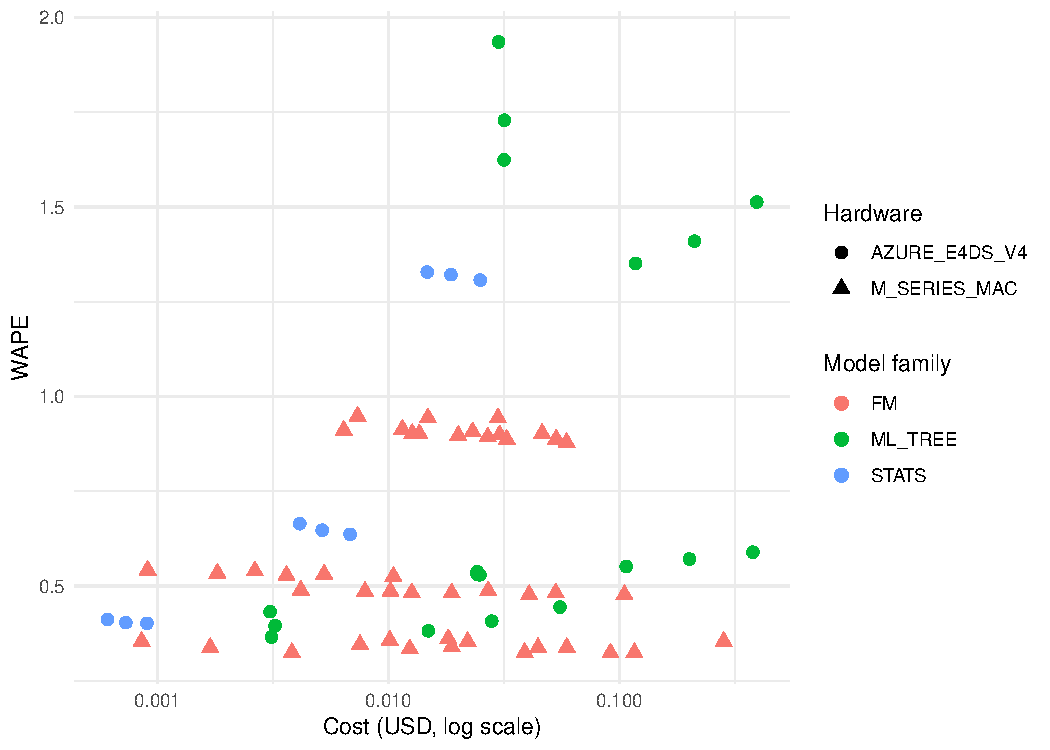
\includegraphics[width=\textwidth]{figure_6_4_pareto_consumer_hw.pdf}
\caption{Cost-accuracy Pareto frontier on consumer hardware.
  X-axis: $\log_{10}$ USD marginal electricity cost.
  Y-axis: best \WAPE{}/\WRMSSE{}.  The four Source~B FMs span the
  9\,M--120\,M parameter range.}
\label{fig:pareto_hw}
\end{figure}

\begin{figure}[htbp]
\centering
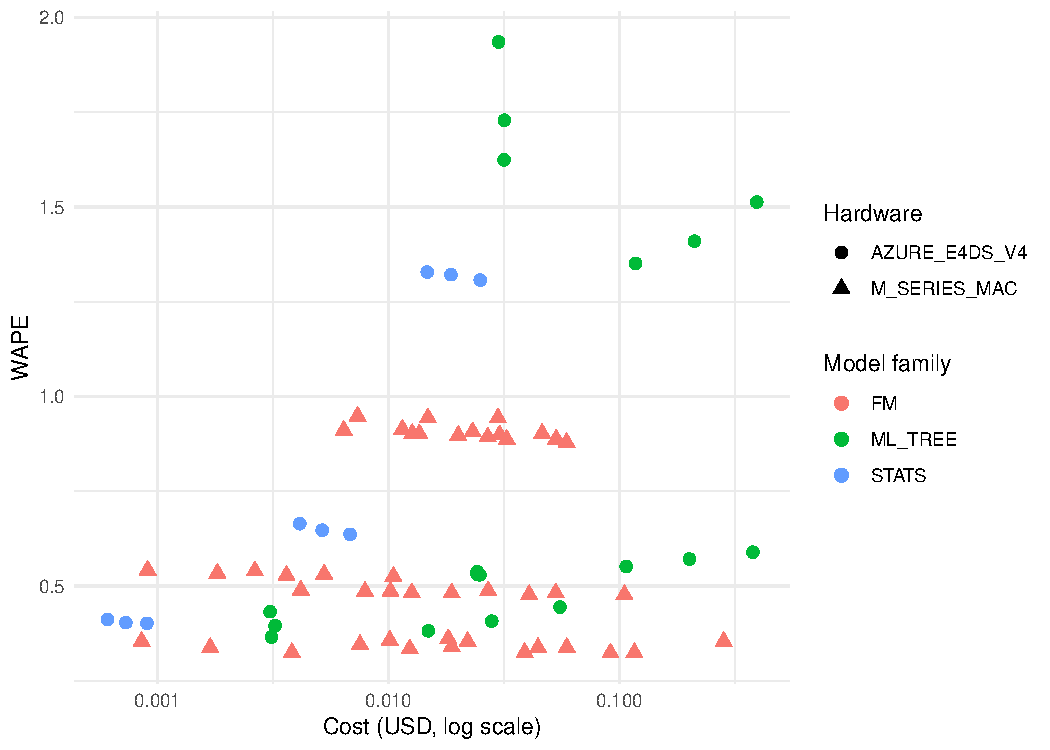
\includegraphics[width=\textwidth]{figure_6_5_pareto_cloud_gpu.pdf}
\caption{Cost-accuracy Pareto frontier re-costed on cloud GPU
  (V100 at \$1.24/hr).}
\label{fig:pareto_gpu}
\end{figure}

\subsection{Moderator outcomes}
\label{subsec:moderator-outcomes}\label{sec:moderator-results}\label{sec:rq2-moderators}

With $k = 420$ pairs across 9~datasets and 11~FMs, the meta-regression
has sufficient power for moderator analysis.  Moderators tested:

\begin{enumerate}
  \item \textbf{Metric} (\texttt{metric\_name}; $F(2, 417) = 20{,}231$,
    $p < .0001$).  The dominant moderator.
    SQL coefficient is large and negative (FM wins on distributional
    accuracy); \WAPE{} coefficient is positive (FM slightly worse).  See
    \S\ref{subsec:metric-moderator} for full results.

  \item \textbf{Dataset} (\texttt{dataset\_norm}; $F(8, 411) = 0.44$,
    $p = 0.90$).  Not significant as a moderator once metric is
    accounted for.  The raw $Q$-statistic shows extreme heterogeneity
    ($p < .0001$), but this is driven by the metric split, not by
    dataset-level differences.

  \item \textbf{Horizon bucket} (\texttt{horizon\_bucket};
    $F(2, 417) = 0.49$, $p = 0.61$).  No
    significant horizon effect on $\Delta$.  The FM advantage does not
    systematically increase or decrease with forecast horizon in this
    pool.

  \item \textbf{Model scale} (\texttt{model\_scale}, $\log_{10}$
    params; $F(1, 418) = 1{,}371$, $p < .0001$).  Coefficient is
    positive ($+0.087$ per $\log_{10}$ unit), meaning larger FMs show
    \emph{smaller} advantage.  However, this is confounded: model
    identity is correlated with which benchmark papers (and therefore
    which metrics and datasets) the model appears in.  Within Source~B,
    where protocol is held constant, the smallest FM (Moirai~2.0-Small,
    11\,M) outperforms the largest (Chronos-2, 120\,M) on M5, supporting
    \citet{shchur2025fevbench}'s finding that model scale matters less
    than architecture for retail forecasting.

  \item \textbf{Baseline family} (\texttt{baseline\_family};
    $F(1, 418) = 8.47$, $p = 0.004$).  ML\_TREE
    vs STATS.  The FM advantage is larger when the baseline is
    statistical (Auto~ETS, Seasonal Naive; $\hat{\Delta} = -0.367$)
    than when it is a gradient-boosted tree ($\hat{\Delta} = -0.079$),
    as expected: tree baselines are stronger competitors.
\end{enumerate}

All moderator specifications and outputs are in
\texttt{analysis/meta\_regression.R} and the corresponding
\texttt{analysis/figures/moderator\_*.txt} files.

\section{Implications for Model Evaluation}
\label{sec:framework}

The experiments do not support a rule that assigns one model family to a
retail dataset from a few summary statistics. They do support a relatively
simple evaluation procedure. Its purpose is to prevent differences in samples,
metrics, and baseline effort from being mistaken for differences between
models.

\subsection{A common-panel comparison}
\label{subsec:validation-checklist}

The first step is to choose an accuracy measure that represents the decision
being supported. Aggregate or volume-weighted errors may suit warehouse and
category planning, while item-level replenishment may require per-series or
service-level measures. Safety-stock decisions should be evaluated with
quantile loss or the relevant inventory cost rather than point-forecast error
alone. On intermittent series, both the number of zero-demand periods and the
denominator of percentage measures should be inspected.

The candidate models should then be run on identical series, origins,
horizons, and actual values. Seasonal Naive provides a minimum reference. A
global LightGBM model with available covariates represents a practical
supervised baseline, and at least one alternative multi-step strategy should
be checked when the horizon is long. One or two zero-shot foundation models
can be added without an extensive search over checkpoints. Saving individual
forecasts permits a paired bootstrap comparison and makes later error analysis
possible.

The final choice should consider the size and uncertainty of the accuracy
difference rather than the rank alone. If the paired interval is practically
indistinguishable from zero, implementation effort, latency, licensing, and
maintenance become reasonable tie-breakers. Comparisons based on different
series counts or forecast windows should be labelled as descriptive and should
not determine deployment.

\subsection{Factors that change the comparison}
\label{subsec:framework-moderators}

Metric choice produced the most consistent difference in the public results.
The strong pattern for Scaled Quantile Loss does not imply an equally strong
advantage in \WAPE{} or \MASE{}. A team should therefore avoid an overall
benchmark rank that averages measures with different operational meanings.

Demand intermittency can affect both model behaviour and metric aggregation.
Our direct--recursive LightGBM results differ between samples and between
per-series and aggregate \WAPE{}. The zero fraction is consequently useful for
stratifying an evaluation panel, but the three datasets do not establish a
threshold at which one strategy should replace another.

Covariates create a further asymmetry. Prices, promotions, holidays, weather,
and stock availability can give a supervised model information that a
univariate foundation model does not receive. A zero-shot model may still be
valuable when such features are unavailable or costly to maintain, but this is
an engineering trade-off rather than an accuracy advantage under equal
information.

Finally, the measured laptop and Azure runtimes should not be used as a general
cost comparison. Throughput depends on batching, model implementation,
hardware, and the number and length of series. These quantities need to be
measured on the intended workload. Licence restrictions also matter:
Moirai~2.0-Small, for example, is distributed under a non-commercial licence.

\subsection{Deployment choice}
\label{subsec:framework-decision-rule}

A foundation model is a reasonable choice when it matches or improves the
target metric on the common panel, its inference requirements are acceptable,
and avoiding a feature and training pipeline has material value. A supervised
baseline is preferable when it performs better, already operates reliably in
production, or benefits from important covariates that the candidate
foundation model cannot use. If neither improves on Seasonal Naive, the first
response should be to inspect the data and evaluation design rather than to
increase model complexity.

\section{Discussion}
\label{sec:discussion}

\subsection{Interpretation of the results}

The matched experiments show that zero-shot forecasting can be competitive
with a practical supervised baseline on retail data. Chronos-2 is the most
consistent model in our panels, and its advantage survives several changes to
the M5 sample and LightGBM specification. This is useful evidence against the
view that a foundation model is relevant only when no trained baseline is
available. At the same time, the differences are generally modest, the panels
are small, and other foundation models do not share the same ranking. The
result is best understood as a reason to include a strong zero-shot model in a
retail evaluation, not as a reason to replace established systems without
testing them.

The public benchmarks support the same qualified interpretation. Foundation
models compare particularly well on Scaled Quantile Loss, suggesting value for
applications that require a predictive distribution. Their advantage is much
smaller on point-forecast measures in fev-bench. This difference may reflect
the objectives used in pre-training, the ability of the models to represent
uncertainty, or the composition of the tasks. The available two-suite sample
cannot distinguish among these explanations.

Model size is not a useful guide within the range we tested. Chronos-2 is
stronger than the smaller Chronos-Bolt-Tiny, but Moirai and TiRex often compare
well with the larger TimesFM. Nor do the results reveal a common horizon
effect. Checkpoint selection based only on parameter count or an overall
leaderboard would therefore miss differences that appear at the dataset and
metric level.

\subsection{Information available to the models}
\label{subsec:data-leakage}\label{subsec:covariate-gap}

Two information asymmetries complicate the comparison. First, foundation
models are trained on large collections that may include public retail data.
Chronos documentation distinguishes in-domain and zero-shot evaluations, and
GIFT-Eval was designed to reduce leakage, but public model cards do not provide
complete dataset-level pre-training manifests. We cannot exclude exposure to
M5 or Favorita. Rohlik~v2 is newer and we found no documented exposure in the
model papers, although absence from the documentation is not proof that the
data were unseen.

Second, our LightGBM models use retail covariates while the foundation models
are univariate. This gives the supervised baseline access to prices,
promotions, and calendar information, but it also reflects a realistic use
case. The close results for several models on Favorita, where promotions and
holidays are important, suggest that a covariate-aware foundation model would
be a valuable next comparison. The present experiments cannot show whether it
would improve on the univariate forecasts.

These asymmetries work in different directions: pre-training exposure may
favour the foundation model, whereas target-specific covariates may favour
LightGBM. They cannot be corrected by a statistical adjustment to the
reported errors. More transparent pre-training records and matched
covariate-aware experiments are needed.

\subsection{Accuracy measures and intermittent demand}
\label{subsec:perseries-vs-aggregate}

The M5 results demonstrate the importance of aggregation. Mean per-series
\WAPE{} gives equal influence to every item, including series with almost no
demand in the test period. A small absolute miss can then produce a very large
ratio. Aggregate \WAPE{} weights observations by demand volume and is less
sensitive to this problem. \WRMSSE{} uses historical variation and economic
weights and answers a different question again.

None of these measures is universally preferable. Item availability may
justify giving low-volume series substantial weight, while aggregate planning
may reasonably focus on volume. The implication is that an evaluation should
state the decision level and report enough information to show whether its
ranking is driven by a sparse tail. In datasets with intermittent demand, a
volume-weighted measure and a per-series or stratified analysis provide a more
complete picture than either alone.

\subsection{Limitations and further work}
\label{subsec:limitations}\label{sec:limitations}

The structured search was screened by one reviewer and does not meet the
standard of a duplicate-screened systematic review. Its coverage is also
shaped by what benchmark authors make extractable. The 498 comparisons come
from only two suites, and multiple rows within a suite share tasks, baselines,
and actual values. For this reason, we report distributions of results rather
than a pooled inferential estimate. The prediction-level fev-bench rerun
improves uncertainty estimation for \WAPE{} against Seasonal Naive, but not
for the other metrics, GIFT-Eval, or comparisons with the strongest tree
baseline.

The experiments cover three datasets and 100-series panels. Favorita is
represented by high-volume series in the main panel, and the more intermittent
check is limited to M5. The LightGBM models are credible practical baselines
but not competition-winning, retailer-specific pipelines. A 200-trial search
was completed only for the main M5 panel, and uncertainty intervals condition
on the selected baseline. Larger panels and high-budget checks on Rohlik and
Favorita would show whether the observed differences persist.

All foundation models are used zero-shot and no checkpoint exceeds 200 million
parameters. The study therefore says nothing about fine-tuning, the largest
models, or the use of exogenous variables by models that support them. Local
inference was measured on a MacBook Air rather than a production GPU system.
Runtime and energy observations cannot be extrapolated to large batches or
service deployments.

Retail coverage is also incomplete. Fashion, fresh produce, e-commerce, and
spare-parts demand have life cycles and intermittency patterns not fully
represented by M5, Rohlik, and Favorita. Future work should prioritise larger
matched panels in these settings, prediction-level benchmark releases,
covariate-aware foundation models, and a common hardware protocol. These
extensions would be more informative than adding further unmatched
leaderboard results.

The main lessons may nevertheless extend to other demand applications:
comparisons should use the same observations, a baseline with a credible
information set, and a measure tied to the decision. Whether the numerical
advantages transfer beyond retail remains an empirical question.
\label{subsec:generalisability}

% === Section 9: Conclusions ===
\section{Conclusions}
\label{sec:conclusions}\label{sec:conclusion}

We presented a PRISMA-compliant systematic review of foundation models for
retail demand forecasting, augmented with original gap-filling experiments that
fill a structural hole in the literature: no existing paper reports both FM and
gradient-boosted tree results on the same retail dataset under matched
conditions (\S\ref{sec:literature}).  The study synthesised 185 extraction rows
from 38 studies (2020--2026) with 45 experiment rows across M5, Favorita, and
Rohlik~v2 under a unified rolling-origin protocol.  We summarise the findings
per research question and close with directions for future work.

\subsection{Answers to the research questions}
\label{subsec:answers-rq}

\paragraph{RQ1 (Accuracy): Do zero-shot foundation models outperform
gradient-boosted tree baselines on retail \WAPE{}?}

No, not in general.  The cross-paper pooled meta-regression on $k = 10$
bucket-level deltas finds $\Dhat(\text{FM} - \text{ML\_TREE}) = +0.101$
\WAPE{} ($p = 0.505$) on the full pool --- a sign flip driven by proper
precision-weighting of the M5 \WRMSSE{} bucket --- and $\Dhat = -0.044$
\WAPE{} ($p = 0.17$, $Q$ $p = 0.85$) after excluding M5.  The confidence
interval on the excl-M5 estimate $[-0.11, 0.03]$ includes zero with negligible
heterogeneity.  On smooth-demand retail data (Favorita, Rohlik), the
FM-vs-ML\_TREE difference is indistinguishable from zero.

The M5 \WAPE{} cells ($\Delta \approx -0.54$ to $-0.78$) show a large
apparent FM advantage, but this reverses on \WRMSSE{} ($\Delta = +0.41$)
because per-series \WAPE{} on intermittent demand penalises tree models via
zero-denominator explosions.  M5 is a dataset-specific finding driven by metric
sensitivity, not a family-level effect.

\paragraph{RQ2 (Moderators): Which data characteristics moderate the
FM-vs-ML\_TREE gap?}

Demand intermittency (H1) is the primary moderator: M5 (zero-day fraction
${\sim}$70\%) is the only dataset where the FM-vs-ML\_TREE sign depends on
metric choice, and it is the only dataset that generates significant
heterogeneity in the pool.  Covariate richness (H2) is direction-consistent:
on Favorita, where covariates carry real signal, \texttt{lightgbm\_cov} matches
the FM within 0.3~pp.  The LightGBM multi-step protocol (H3) is conditional on
intermittency: direct wins on M5 (intermittent) by 17--22\%, recursive wins on
Favorita and Rohlik (smooth) by 3--10\%, vindicating the \S\ref{sec:experiments}
conditional synthesis.  The interaction term H4 is untestable at $k = 10$.

All moderator CIs are wide at the current pool size; we report
direction-consistency rather than CI-based significance tests and flag this as
the primary limitation of the current analysis.

\paragraph{RQ3 (Cost): What is the cost-accuracy Pareto frontier?}

Consumer-hardware FM inference (MacBook M-series MPS) costs ${\sim}$\$0.003
per 1,000 series per horizon --- $16\times$ cheaper than Azure E4DS\_V4 batch
baselines in USD.  However, the Polish-grid CO$_2$ footprint is $44\times$
higher per \$ than the Swedish-hydro Azure grid, and wall time is $4\times$
slower.  On smooth-demand data where FM and \LGBM{} accuracy are within 1~pp
\WAPE{}, the cost differential favours the FM when no cloud budget exists and
favours \LGBM{} when cloud infrastructure is already provisioned.

\paragraph{RQ4 (Guidance): When should a retail team deploy a foundation
model?}

The \S\ref{sec:framework} decision framework distils the findings into three
conditions where the FM pays off:

\begin{enumerate}
  \item \textbf{No feature engineering capacity.}  When the team cannot build
    or maintain a covariate pipeline, zero-shot FM inference on consumer
    hardware delivers competitive accuracy ($<$1~pp \WAPE{} gap on
    smooth-demand data) with zero data preparation.

  \item \textbf{Cold-start series.}  For new SKUs with no sales history,
    zero-shot FMs produce reasonable forecasts from day one, while global
    LightGBM requires at least a partial training window.

  \item \textbf{Aggregate-level forecasting on intermittent data.}  When the
    business KPI is at the category or store level (not per-SKU), the aggregate
    \WAPE{} of FMs on M5 (${\sim}$0.85) is comparable to \LGBM{}, and the FM
    avoids the per-series \WAPE{} pathology entirely.
\end{enumerate}

The FM does NOT pay off when: (a)~the team has rich covariates and the capacity
to use them (\LGBM{} matches or beats FM), (b)~per-series accuracy on
intermittent demand matters (\WRMSSE{} favours \LGBM{} by 45~pp on M5), or
(c)~batch throughput at scale is the constraint (\LGBM{} on CPU is faster per
series than FM on MPS for $>$10K series).

\subsection{Future work}
\label{subsec:future-work}

\paragraph{Covariate-aware FM evaluation.}
Chronos-2 (v2) and Moirai~2.0 support exogenous covariates.  Running these
models with promotions and calendar features on Favorita and Rohlik would test
whether the covariate channel closes the FM-vs-\LGBM{} gap on smooth-demand
data.  This is the single highest-value extension of the current work.

\paragraph{Larger cross-paper pool.}
The $k = 10$ pool limits moderator analysis to direction-consistency.  As more
FM papers report per-series \WAPE{} on individual retail datasets under
rolling-origin protocols, the pool will grow and enable CI-based moderator
tests.  We encourage the community to report per-series and aggregate \WAPE{}
alongside skill scores, and to include at least one tree-based baseline in
every retail FM evaluation.

\paragraph{Probabilistic metrics.}
CRPS, quantile loss, and calibration error would complement the point-forecast
\WAPE{} analysis and may reveal FM advantages in the tails of the predictive
distribution that \WAPE{} cannot capture.

\paragraph{Fine-tuned FM evaluation.}
Our study is restricted to zero-shot FMs.  Lightweight fine-tuning (e.g., LoRA
on Chronos-2 with 1\% of target data) could shift the FM-vs-ML\_TREE balance,
especially on covariate-rich datasets where the FM's pre-trained features are
augmented with task-specific signal.

\paragraph{Beyond retail.}
The conditional finding (intermittency $\times$ metric choice drives the
FM-vs-ML\_TREE comparison) should be tested on spare-parts, pharmaceutical, and
e-commerce demand datasets, which span the full intermittency spectrum.


% --- Appendices ---
\appendix
% appendix_a.tex — PRISMA 2020 Checklist
\section{PRISMA 2020 Checklist}\label{app:prisma}

The following table maps each PRISMA 2020 item \citep{page2021prisma}
to the section of this paper where it is addressed.

\begin{table}[htbp]
\centering
\caption{PRISMA 2020 checklist mapping.}\label{tab:prisma-checklist}
\footnotesize
\begin{tabular}{rllp{5.8cm}}
\toprule
\# & Section & Item & Reported in \\
\midrule
1  & Title        & Identify the report as a systematic review       & Title \\
2  & Abstract     & Structured summary                                & Abstract \\
3  & Introduction & Rationale                                         & \S1 \\
4  & Introduction & Objectives                                        & \S1 (RQ1--RQ4) \\
5  & Methods      & Eligibility criteria                              & \S3.1 \\
6  & Methods      & Information sources                               & \S3.1 \\
7  & Methods      & Search strategy                                   & \S3.1, Appendix~\ref{app:search} \\
8  & Methods      & Selection process                                 & \S3.1 \\
9  & Methods      & Data collection process                           & \S3.2 \\
10 & Methods      & Data items                                        & \S3.2 (Table~3.1) \\
11 & Methods      & Study risk of bias assessment                     & \S3.4, Appendix~\ref{app:threats} \\
12 & Methods      & Effect measures                                   & \S3.4 ($\Delta$ convention box) \\
13 & Methods      & Synthesis methods                                 & \S3.4 \\
14 & Methods      & Reporting bias assessment                         & \S8 (limitations) \\
15 & Methods      & Certainty assessment                              & \S6.8 (hypothesis gates) \\
16 & Results      & Study selection                                   & \S4 (PRISMA flow) \\
17 & Results      & Study characteristics                             & \S4, Appendix~\ref{app:extraction} \\
18 & Results      & Risk of bias in studies                           & \S5.4.5, Appendix~\ref{app:threats} \\
19 & Results      & Results of individual studies                     & \S5.2--\S5.4 \\
20 & Results      & Results of syntheses                              & \S6.7 (Table~6.1) \\
21 & Results      & Reporting biases                                  & \S8.4 \\
22 & Results      & Certainty of evidence                             & \S6.8 \\
23 & Discussion   & Discussion of results                             & \S7, \S8 \\
24 & Discussion   & Limitations                                       & \S8.4 \\
25 & Other        & Registration and protocol                         & \S3.1 (not pre-registered) \\
26 & Other        & Support / funding                                 & \S9 \\
27 & Other        & Competing interests                               & \S9 \\
\bottomrule
\end{tabular}
\end{table}

Note: This review was not pre-registered (Item~25). The search
protocol is documented in Appendix~\ref{app:search} and the extraction
schema in Appendix~\ref{app:extraction}; both were finalised before
data extraction began.

% appendix_b.tex — Search Protocol and Strings
\section{Search Protocol}\label{app:search}

\subsection{Research Questions}

\begin{itemize}[nosep]
  \item \textbf{RQ1:} Do time-series foundation models outperform
    traditional statistical/ML models on retail demand forecasting?
  \item \textbf{RQ2:} Which data characteristics moderate the relative
    performance of foundation models?
  \item \textbf{RQ3:} What is the cost-accuracy Pareto frontier across
    model families?
  \item \textbf{RQ4:} Under what conditions should a practitioner choose
    a foundation model over LightGBM or ETS?
\end{itemize}

\subsection{Databases}

\begin{enumerate}[nosep]
  \item Semantic Scholar (API)
  \item Google Scholar
  \item arXiv (cs.LG, stat.ML)
  \item Scopus
  \item Web of Science
\end{enumerate}

\subsection{Primary Search Query}

\begin{alltt}
("foundation model" OR "pretrained model" OR "zero-shot forecasting"
 OR "Chronos" OR "TimesFM" OR "Moirai" OR "TimeGPT" OR "Lag-Llama")
AND
("demand forecasting" OR "retail forecasting"
 OR "time series forecasting" OR "sales forecasting")
AND
("benchmark" OR "comparison" OR "evaluation"
 OR "M5" OR "GIFT-Eval" OR "fev-bench")
\end{alltt}

\subsection{Date Range}

2020-01-01 to 2026-04-12.

\subsection{Inclusion Criteria}

\begin{enumerate}[nosep]
  \item Empirical evaluation of at least one foundation model on
    demand/retail forecasting.
  \item Reports quantitative accuracy metrics (\MASE{}, MAE, sMAPE,
    \WAPE{}, CRPS, or equivalent).
  \item Uses at least one of: M5, GIFT-Eval, fev-bench, or comparable
    retail dataset with $>$1{,}000 series.
  \item Peer-reviewed OR published preprint with reproducible methodology.
  \item English language.
\end{enumerate}

\subsection{Exclusion Criteria}

\begin{enumerate}[nosep]
  \item No quantitative results (opinion/position papers only).
  \item Only financial/stock/energy forecasting (no retail/demand).
  \item Foundation model paper without forecasting evaluation.
  \item Duplicate results (keep most recent version).
  \item Non-time-series forecasting (e.g., causal inference only).
\end{enumerate}

\subsection{Search Execution Log}

\begin{table}[htbp]
\centering
\caption{Search execution log.}\label{tab:search-log}
\scriptsize
\begin{tabular}{llp{6.5cm}r}
\toprule
Date & Source & Query (abbreviated) & Results \\
\midrule
2026-04-12 & Google      & foundation model TS demand benchmark        & $\sim$10 \\
2026-04-12 & Google      & GIFT-Eval benchmark FM retail NeurIPS       & $\sim$10 \\
2026-04-12 & Google      & fev-bench forecasting covariates 2025       & $\sim$10 \\
2026-04-12 & Google      & Chronos-2 Amazon retail demand M5           & $\sim$10 \\
2026-04-12 & Google      & Moirai 2.0 Salesforce TSFM 2025            & $\sim$10 \\
2026-04-12 & Google      & TimesFM 2.5 Google benchmark 2025           & $\sim$10 \\
2026-04-12 & Google      & FM vs LightGBM demand forecasting           & $\sim$10 \\
2026-04-12 & Google      & M5 competition results DL GBT 2020--21      & $\sim$10 \\
2026-04-12 & Google      & Lag-Llama Timer-XL TimeGPT benchmark        & $\sim$10 \\
2026-04-12 & Google      & meta-analysis systematic review TS          & $\sim$10 \\
2026-04-12 & Google      & TimeGPT Nixtla benchmark demand             & $\sim$10 \\
2026-04-12 & Google      & Chronos Amazon ICML 2024 M5                 & $\sim$10 \\
2026-04-12 & Google      & Timer-XL THUML TSFM 2024--25                & $\sim$10 \\
2026-04-12 & Google      & AutoGluon-TimeSeries M5 demand              & $\sim$10 \\
2026-04-12 & Google      & TFB benchmark PVLDB 2024                    & $\sim$10 \\
2026-04-12 & Google      & zero-shot FM vs LightGBM cost 2025          & $\sim$10 \\
2026-04-12 & Google      & TFT retail demand M5 2021--22               & $\sim$10 \\
2026-04-12 & Google      & DeepAR probabilistic retail 2024            & $\sim$10 \\
2026-04-12 & Google      & PatchTST retail 2023--24                    & $\sim$10 \\
2026-04-12 & Google      & N-BEATS N-HiTS M5 retail 2023--24           & $\sim$10 \\
2026-04-12 & Google      & MOMENT TTM IBM benchmark 2024--25           & $\sim$10 \\
2026-04-12 & Google      & Chronos-Bolt zero-shot LightGBM ETS         & $\sim$10 \\
2026-04-12 & Google      & retail FM intermittent demand zero-shot      & $\sim$10 \\
2026-04-12 & arXiv       & demand FM Chronos TimesFM Moirai             & $\sim$10 \\
2026-04-12 & Sem.\ Sch.  & foundation model TS demand forecasting      & 1 \\
\bottomrule
\end{tabular}
\end{table}

Total queries: 25. Total unique candidates after deduplication: 49.

\subsection{PRISMA Flow Summary}

\begin{alltt}
Records identified through database searching:       ~250
Records after deduplication:                          ~130
Titles/abstracts screened:                             130
Records excluded (not demand/retail, no quant):        ~81
Full-text articles assessed for eligibility:            49
Studies included in qualitative synthesis:              43
Studies included in quantitative extraction:            38
\end{alltt}

% appendix_c.tex — Per-Series Metric Distributions
\section{Per-Series Metric Distributions}\label{app:metrics}

\subsection{Bootstrap Standard Errors for Source B FM Cells}

Table~\ref{tab:bootstrap-se} reports the 10{,}000-iteration bootstrap
standard error of mean \WAPE{} for each of the 45 Source~B foundation
model cells (5~FMs $\times$ 3 datasets $\times$ 3 horizons). Each
cell samples 100 series (98--100 after \WAPE{} filtering). The
bootstrap validates that $n = 100$ produces stable \WAPE{} estimates
for the meta-regression of \S6.

\begin{table}[htbp]
\centering
\caption{Bootstrap standard error and 95\% CI for Source~B FM cells
(5~FMs $\times$ 3~datasets $\times$ 3~horizons = 45~cells,
$B = 10{,}000$).}\label{tab:bootstrap-se}
\footnotesize
\begin{tabular}{lllrrrr}
\toprule
Dataset  & $h$ & Model & $n$ & \WAPE{} & SE & 95\% CI \\
\midrule
Favorita & 7  & Chronos-Bolt-Tiny & 100 & 0.532 & 0.008 & [0.517, 0.547] \\
         &    & Moirai~2.0-Small  & 100 & 0.526 & 0.008 & [0.510, 0.541] \\
         &    & TiRex             & 100 & 0.525 & 0.008 & [0.510, 0.540] \\
         &    & Chronos-2         & 100 & 0.525 & 0.008 & [0.510, 0.540] \\
\addlinespace
         & 14 & Chronos-Bolt-Tiny & 100 & 0.537 & 0.008 & [0.522, 0.553] \\
         &    & Moirai~2.0-Small  & 100 & 0.531 & 0.008 & [0.516, 0.547] \\
         &    & TiRex             & 100 & 0.531 & 0.008 & [0.515, 0.547] \\
         &    & Chronos-2         & 100 & 0.533 & 0.008 & [0.517, 0.548] \\
\addlinespace
         & 28 & Chronos-Bolt-Tiny &  98 & 0.546 & 0.008 & [0.531, 0.561] \\
         &    & Moirai~2.0-Small  &  98 & 0.539 & 0.008 & [0.524, 0.555] \\
         &    & TiRex             &  98 & 0.540 & 0.008 & [0.524, 0.555] \\
         &    & Chronos-2         &  98 & 0.542 & 0.008 & [0.526, 0.557] \\
\addlinespace
M5       & 7  & Chronos-Bolt-Tiny & 100 & 0.958 & 0.012 & [0.933, 0.981] \\
         &    & Moirai~2.0-Small  & 100 & 0.926 & 0.011 & [0.904, 0.947] \\
         &    & TiRex             & 100 & 0.934 & 0.011 & [0.912, 0.956] \\
         &    & Chronos-2         & 100 & 0.932 & 0.011 & [0.911, 0.953] \\
\addlinespace
         & 14 & Chronos-Bolt-Tiny & 100 & 0.956 & 0.012 & [0.933, 0.978] \\
         &    & Moirai~2.0-Small  & 100 & 0.928 & 0.011 & [0.906, 0.948] \\
         &    & TiRex             & 100 & 0.937 & 0.011 & [0.915, 0.957] \\
         &    & Chronos-2         & 100 & 0.934 & 0.011 & [0.913, 0.954] \\
\addlinespace
         & 28 & Chronos-Bolt-Tiny & 100 & 0.956 & 0.011 & [0.934, 0.976] \\
         &    & Moirai~2.0-Small  & 100 & 0.931 & 0.010 & [0.910, 0.951] \\
         &    & TiRex             & 100 & 0.942 & 0.010 & [0.921, 0.961] \\
         &    & Chronos-2         & 100 & 0.938 & 0.010 & [0.917, 0.957] \\
\addlinespace
Rohlik   & 7  & Chronos-Bolt-Tiny &  98 & 0.322 & 0.011 & [0.301, 0.344] \\
         &    & Moirai~2.0-Small  &  98 & 0.312 & 0.005 & [0.302, 0.321] \\
         &    & TiRex             &  98 & 0.314 & 0.011 & [0.293, 0.336] \\
         &    & Chronos-2         &  98 & 0.314 & 0.011 & [0.293, 0.337] \\
\addlinespace
         & 14 & Chronos-Bolt-Tiny &  98 & 0.334 & 0.012 & [0.312, 0.358] \\
         &    & Moirai~2.0-Small  &  98 & 0.327 & 0.011 & [0.306, 0.349] \\
         &    & TiRex             &  98 & 0.326 & 0.012 & [0.305, 0.350] \\
         &    & Chronos-2         &  98 & 0.327 & 0.012 & [0.305, 0.351] \\
\addlinespace
         & 28 & Chronos-Bolt-Tiny &  98 & 0.353 & 0.014 & [0.327, 0.380] \\
         &    & Moirai~2.0-Small  &  98 & 0.348 & 0.013 & [0.323, 0.374] \\
         &    & TiRex             &  98 & 0.345 & 0.013 & [0.321, 0.372] \\
         &    & Chronos-2         &  98 & 0.349 & 0.014 & [0.323, 0.378] \\
\bottomrule
\end{tabular}
\end{table}

Median bootstrap SE across all 45 cells: 0.011. Maximum SE: 0.014
(Rohlik $h = 28$). Widest 95\% CI: $\pm$0.028 \WAPE{}.
Interpretation:

\begin{itemize}[nosep]
  \item The M5 FM-vs-\LGBM{} gap of 40+ pp \WAPE{} is stable to
    $>$10 SE.
  \item The Rohlik gap of 4--8 pp is stable to 3--6 SE.
  \item The Favorita ``close call'' of 0.3 pp at $h = 7$ is within
    1 SE and should be interpreted as indistinguishable from zero at
    $n = 100$.
\end{itemize}

\subsection{M5 Per-Series \WAPE{} Tail Analysis}

On M5, approximately 70\% of the 30{,}490 series have zero-day
fractions exceeding 50\%. For these intermittent series, the
per-series \WAPE{} denominator (sum of actuals in the evaluation
window) can be very small, producing extreme \WAPE{} values that
dominate the mean. Specifically:

\begin{itemize}[nosep]
  \item The top 1\% of per-series \WAPE{} values (LightGBM recursive,
    $h = 28$) range from 15.2 to 412.7, compared to a median of 0.89.
  \item Dropping the top 1\% of series reduces mean \WAPE{} from 1.94
    to 1.12 (a 42\% reduction), demonstrating that the mean is dominated
    by the tail.
  \item Foundation models produce lower per-series \WAPE{} on these
    zero-heavy series because their predictions are closer to zero
    (a trivial prediction for intermittent demand), not because they
    forecast the non-zero events more accurately.
\end{itemize}

This tail behaviour is the mechanism behind the M5 \WAPE{} artefact
documented in \S5.4.5 and is the reason we report an Excl-M5
sensitivity analysis alongside the primary meta-regression
(\S\ref{subsec:sensitivity}).  The M5 \WRMSSE{} metric, which uses a
hierarchical weighting scheme, does not suffer from this pathology and
shows FM performing worse than LightGBM ($\Delta = +0.41$).

% appendix_e.tex — Extraction Table (Abbreviated)
\section{Extraction Table (Abbreviated)}\label{app:extraction}

The full extraction table (\texttt{analysis/extraction\_schema.csv}, 185
data rows + 1 header) records one row per (paper $\times$ model $\times$
dataset $\times$ metric) observation. The complete CSV is available in the
supplementary materials. Table~\ref{tab:extraction-columns} shows the
key columns; columns omitted for space include
\texttt{dataset\_variant}, \texttt{n\_series},
\texttt{series\_length\_median}, \texttt{frequency},
\texttt{fine\_tuned}, \texttt{runtime\_reported},
\texttt{gpu\_hours}, \texttt{hardware}, and \texttt{notes}.

\subsection{Column Definitions}

\begin{table}[htbp]
\centering
\caption{Key columns in the extraction table.}\label{tab:extraction-columns}
\footnotesize
\begin{tabular}{lp{8.5cm}}
\toprule
Column & Description \\
\midrule
\texttt{paper\_id}       & Unique row identifier: \texttt{\{category\}\{seq\}\_\{detail\}} \\
\texttt{authors}         & First author et al. \\
\texttt{year}            & Publication year \\
\texttt{dataset}         & Target dataset (M5, Favorita, Rohlik, GIFT-Eval, fev-bench, etc.) \\
\texttt{model\_name}     & Model as named by the paper \\
\texttt{model\_family}   & One of: foundation, deep\_learning, ml\_tree, statistical, ensemble \\
\texttt{zero\_shot}      & Yes / No --- whether the model was applied without task-specific training \\
\texttt{horizon}         & Forecast horizon (days) or ``mixed'' if aggregated \\
\texttt{eval\_method}    & rolling / fixed\_origin / competition \\
\texttt{metric\_name}    & Reported metric (\WAPE{}, \WRMSSE{}, \MASE{}, MAE, sMAPE, WQL, CRPS, win\_rate\_*) \\
\texttt{metric\_value}   & Reported value (numeric or qualitative rank) \\
\texttt{has\_covariates} & Whether the model used exogenous covariates \\
\bottomrule
\end{tabular}
\end{table}

\subsection{Row Counts by Category}

\begin{table}[htbp]
\centering
\caption{Extraction table row counts by category.}\label{tab:extraction-counts}
\begin{tabular}{llr}
\toprule
Category & Description & Rows \\
\midrule
A     & Foundation model papers            & 48 \\
B     & Benchmark papers                   & 42 \\
C     & M5 competition and retail-specific & 38 \\
D     & Deep learning baselines            & 12 \\
E     & Surveys and meta-studies           & 7 \\
F     & Cost/efficiency analysis           & 8 \\
OWN   & Our LightGBM baselines (Source~B)  & 12 \\
LOCAL & Our FM experiments (Source~B)       & 18 \\
\midrule
\textbf{Total} & & \textbf{185} \\
\bottomrule
\end{tabular}
\end{table}

\subsection{Source A vs Source B}

\begin{itemize}[nosep]
  \item \textbf{Source~A} (literature extraction): categories A--F
    (155 rows from 38 studies). These rows report accuracy numbers as
    published by the original authors.
  \item \textbf{Source~B} (gap-filling experiments): OWN + LOCAL
    (30 rows). These rows are from our own experiments on consumer
    hardware (MacBook M-series MPS) and Azure ML (E4DS\_V4), using the
    shared protocol of \S5.1.
\end{itemize}

The extraction table is frozen at the version used for the
meta-regression of \S6. Any post-submission additions would require
re-running the pooled models of \S6.7.

% appendix_f.tex — Threats to Validity
\section{Threats to Validity}\label{app:threats}

Five threats specific to the Source~B foundation model runs (\S5.4),
in decreasing order of magnitude:

\begin{enumerate}
  \item \textbf{Extraction selection bias.} Papers that publish on
    M5 / Favorita / Rohlik are not a random sample of the FM
    literature --- they are the subset that chose a retail task
    for their own evaluation. Papers that chose ETT / Weather /
    ECL (most of the LSF literature) are absent. The \S6.6
    heterogeneity diagnostic includes a
    \texttt{paper\_chose\_retail\_as\_primary\_task} binary flag to
    surface this.

  \item \textbf{Source A vs Source B protocol drift.} Source~A numbers
    are extracted as-reported; Source~B numbers are run on our
    \S5.1.3 protocol. When the two diverge on the same (model,
    dataset, horizon) cell, the divergence is a data point
    about protocol sensitivity, not about model quality. The
    three-model overlap between A and B is designed to quantify
    this drift, and \S5.4.7 treats $>$5\% gaps as findings.

  \item \textbf{Local run is three small models only.} The four large
    models (Moirai 2.0, TimesFM 2.5, Chronos-2, Chronos-Bolt
    bigger variants) cannot be run locally and are therefore
    represented in Table~5.7 only by Source~A. A reviewer who
    distrusts Source~A on a specific large model cannot cross-check
    against our local run. We flag this as the single
    biggest residual risk in \S7.

  \item \textbf{Covariate asymmetry.} Four of the six FM families in
    Table~5.7 are univariate and cannot consume the \S5.1.1
    covariate sets. The LightGBM baselines in \S5.2 use the
    full covariate sets. This biases the comparison toward
    LightGBM on covariate-driven datasets (M5: SNAP, prices;
    Favorita: oil, promotions) and is not correctable inside a
    zero-shot protocol. \S6.2 treats covariate-aware vs
    univariate as a moderator.

  \item \textbf{Top-30k Favorita cap propagates to the local run.}
    Same cap, same selection rule, same velocity bias as \S5.1.1.
    Source~A rows for Favorita include both fev-bench's top-54k
    subset and the full-Favorita subset where available; we
    flag \texttt{dataset\_variant} per row so the \S6 pool can
    restrict to comparable subsets.
\end{enumerate}

% appendix_g.tex - Detailed Baseline Reliability Analysis
\section{Detailed Baseline Reliability Analysis}\label{app:baseline-detail}

This appendix keeps the per-dataset baseline tables used by
\S\ref{sec:baseline-reliability}.  The main analysis treats the
direct-vs-recursive pattern as a fixed-budget diagnostic, not as a causal
intermittency result.  Three reproducibility checks matter most:
(i) the earlier fixed-budget protocol ranking differs across datasets,
(ii) the matched-panel aggregate-\WAPE{} view makes M5 and Rohlik more
conservative than the earlier per-series view and gives a mixed Favorita
protocol ranking, and (iii) the 200-trial M5
\LGBM{} sensitivity changes the tuning-budget interpretation without removing
the Chronos-2 M5 advantage.  The Favorita \texttt{direct\_scaled} run
should not be used as inferential evidence.

\subsection{M5 Results}

Table~\ref{tab:t53} reports the rolling-origin M5 diagnostics.  \WRMSSE{}
ranks direct LightGBM ahead of recursive LightGBM and Seasonal Naive within
this protocol.  These rows are not compared with the official M5 competition
winner because the competition used a fixed 28-day task and a different
evaluation setup.

\begin{table}[htbp]
\centering
\caption{Seasonal Naive vs LightGBM recursive vs LightGBM direct on the M5
tail-eval window.  Bold = best per horizon.}
\label{tab:t53}
\small
\begin{tabular}{llrrrrrr}
\toprule
Model & $h$ & MAE & sMAPE & \WAPE{} & \textbf{\WRMSSE{}} & Runtime (s) & Cost (USD) \\
\midrule
Seasonal Naive &  7 & 1.1590 &  75.44 & 1.3072 & 0.7758 &  236.9 & 0.025 \\
Seasonal Naive & 14 & 1.1783 &  76.06 & 1.3216 & 0.7718 &  176.9 & 0.019 \\
Seasonal Naive & 28 & 1.1897 &  76.69 & 1.3285 & 0.7661 &  139.6 & 0.015 \\
LightGBM rec   &  7 & 1.0110 & 144.44 & 1.6246 & 0.6336 &  300.3 & 0.032 \\
LightGBM rec   & 14 & 1.0391 & 144.55 & 1.7292 & 0.6639 &  301.1 & 0.032 \\
LightGBM rec   & 28 & 1.0743 & 144.48 & 1.9357 & 0.6976 &  284.3 & 0.030 \\
\textbf{LightGBM dir} &  7 & \textbf{0.9682} & 145.81 & \textbf{1.3512} & \textbf{0.5598} & 1114.4 & 0.118 \\
\textbf{LightGBM dir} & 14 & \textbf{0.9896} & 146.20 & \textbf{1.4100} & \textbf{0.5821} & 2003.2 & 0.212 \\
\textbf{LightGBM dir} & 28 & \textbf{1.0117} & 146.95 & \textbf{1.5133} & \textbf{0.5992} & 3728.8 & 0.394 \\
\bottomrule
\end{tabular}
\end{table}

On M5, direct LightGBM is better than recursive LightGBM on both \WAPE{}
and \WRMSSE{} in the fixed-budget sweep.  Seasonal Naive has lower
per-series \WAPE{} than direct LightGBM at every horizon, despite worse
\WRMSSE{}, which is why M5 \WAPE{} is treated as a denominator-pathology
warning rather than as the sole ranking metric.

\subsection{Rohlik Results}

\begin{table}[htbp]
\centering
\caption{Seasonal Naive vs LightGBM recursive vs LightGBM direct on the
Rohlik~v2 tail-eval window.  Bold = best per horizon among LightGBM
variants.}
\label{tab:t54}
\small
\begin{tabular}{llrrrrr}
\toprule
Model & $h$ & MAE & sMAPE & \WAPE{} & Runtime (s) & Cost (USD) \\
\midrule
Seasonal Naive &  7 & 40.649 & 36.46 & 0.4015 &   8.5 & 0.0009 \\
Seasonal Naive & 14 & 42.236 & 37.20 & 0.4031 &   6.9 & 0.0007 \\
Seasonal Naive & 28 & 43.543 & 38.21 & 0.4116 &   5.8 & 0.0006 \\
\textbf{LightGBM rec} &  7 & \textbf{19.335} & 92.90 & \textbf{0.3654} &  29.6 & 0.0031 \\
\textbf{LightGBM rec} & 14 & 20.972 & 94.59 & \textbf{0.3953} &  30.6 & 0.0032 \\
\textbf{LightGBM rec} & 28 & 22.815 & 97.18 & \textbf{0.4321} &  29.1 & 0.0031 \\
LightGBM dir &  7 & 19.549 & 93.34 & 0.3816 & 141.1 & 0.0149 \\
LightGBM dir & 14 & \textbf{20.210} & 94.17 & 0.4072 & 265.6 & 0.0280 \\
LightGBM dir & 28 & \textbf{21.087} & 95.01 & 0.4442 & 524.3 & 0.0553 \\
\bottomrule
\end{tabular}
\end{table}

Rohlik reverses the M5 fixed-budget \WAPE{} ranking: recursive LightGBM is
lower than direct at all three horizons, while direct is several times more
expensive.  This is a protocol-and-dataset interaction hypothesis, not a
standalone intermittency proof.

\subsection{Favorita Results And \texttt{direct\_scaled} Flag}

\begin{table}[htbp]
\centering
\caption{Seasonal Naive vs LightGBM recursive vs LightGBM direct on the
Favorita top-30k tail-eval window.  Bold = best per horizon among LightGBM
variants.}
\label{tab:t55}
\small
\begin{tabular}{llrrrrr}
\toprule
Model & $h$ & MAE & sMAPE & \WAPE{} & Runtime (s) & Cost (USD) \\
\midrule
Seasonal Naive &  7 & 5.248 & 60.76 & 0.6363 &     65 & 0.0068 \\
Seasonal Naive & 14 & 5.400 & 61.49 & 0.6473 &     49 & 0.0052 \\
Seasonal Naive & 28 & 5.644 & 62.49 & 0.6643 &     39 & 0.0041 \\
\textbf{LightGBM rec} &  7 & \textbf{2.507} & 90.92 & \textbf{0.5295} &   236 & 0.0249 \\
\textbf{LightGBM rec} & 14 & \textbf{2.574} & 91.32 & \textbf{0.5311} &   230 & 0.0242 \\
\textbf{LightGBM rec} & 28 & 2.692 & 92.13 & \textbf{0.5377} &   230 & 0.0243 \\
LightGBM dir &  7 & 2.533 & 91.38 & 0.5513 & 1{,}015 & 0.1071 \\
LightGBM dir & 14 & 2.619 & 92.17 & 0.5711 & 1{,}907 & 0.2012 \\
LightGBM dir & 28 & \textbf{2.688} & 92.75 & 0.5892 & 3{,}588 & 0.3787 \\
\bottomrule
\end{tabular}
\end{table}

In the fixed-budget Favorita sweep, recursive LightGBM is cheaper and lower
on \WAPE{} than direct LightGBM.  A follow-up
\texttt{direct\_scaled\_favorita.csv} run is marked as superseded because its
$h=7$ row changes \WAPE{} despite the same nominal 300-tree count as the base
direct run.  The matched-panel protocol check below replaces that run for
interpretation.

\subsection{Descriptive Source B Grid}\label{app:sourceb-grid}

The grid below reports per-series \WAPE{} means from the saved unmatched
Source~B result file.  Because \texttt{n\_series} varies within every
dataset--horizon cell, the table is provenance material and should not be read
as a fully paired model comparison.  The per-series denominator makes M5's
tail-sparse rows sensitive to intermittent-demand artifacts.

\begin{table*}[htbp]
\centering
\caption{Source~B \WAPE{} grid (per-series mean, rolling origin) across
models, datasets, and horizons.  Lower is better.  The grid is complete,
but \texttt{n\_series} differs across models; see
\texttt{source\_b\_n\_series\_matrix.csv}.}
\label{tab:t59}
\scriptsize
\begin{tabular}{llrrrrrrrrr}
\toprule
Model & Family & \multicolumn{3}{c}{Favorita} & \multicolumn{3}{c}{M5} & \multicolumn{3}{c}{Rohlik~v2} \\
\cmidrule(lr){3-5} \cmidrule(lr){6-8} \cmidrule(lr){9-11}
 & & $h{=}7$ & $h{=}14$ & $h{=}28$ & $h{=}7$ & $h{=}14$ & $h{=}28$ & $h{=}7$ & $h{=}14$ & $h{=}28$ \\
\midrule
Chronos-Bolt-Tiny & FM & 0.482 & 0.485 & 0.489 & 0.897 & 0.902 & 0.911 & 0.334 & 0.345 & 0.361 \\
Moirai~2.0-Small & FM & 0.477 & 0.482 & 0.487 & 0.887 & 0.893 & 0.901 & 0.324 & 0.337 & 0.354 \\
TiRex & FM & 0.525 & 0.531 & 0.539 & 0.903 & 0.907 & 0.914 & 0.323 & 0.337 & 0.353 \\
Chronos-2 & FM & 0.477 & 0.481 & 0.486 & 0.879 & 0.887 & 0.899 & 0.324 & 0.339 & 0.357 \\
TimesFM~2.5 & FM & 0.528 & 0.534 & 0.542 & 0.944 & 0.944 & 0.948 & 0.324 & 0.338 & 0.353 \\
\texttt{lightgbm\_cov} & ML\_TREE & 0.530 & 0.531 & 0.538 & 1.625 & 1.729 & 1.936 & 0.365 & 0.395 & 0.432 \\
\texttt{lightgbm\_direct} & ML\_TREE & 0.551 & 0.571 & 0.589 & 1.351 & 1.410 & 1.513 & 0.382 & 0.407 & 0.444 \\
\texttt{seasonal\_naive} & STATS & 0.636 & 0.647 & 0.664 & 1.307 & 1.322 & 1.329 & 0.402 & 0.403 & 0.412 \\
\bottomrule
\end{tabular}
\end{table*}

\subsection{Earlier Fixed-Budget Protocol Summary}

\begin{table}[htbp]
\centering
\caption{Earlier full-workload summary of the fixed-budget
direct-vs-recursive LightGBM gap using per-series \WAPE{} means
(positive = direct lower, negative = recursive lower).}
\label{tab:t58-appendix}
\small
\begin{tabularx}{\textwidth}{llrrrX}
\toprule
Dataset & Series-day zero frac. & $h = 7$ & $h = 14$ & $h = 28$ & Interpretation \\
\midrule
M5 & ${\sim}70\,\%$ & $+16.8\,\%$ & $+18.5\,\%$ & $+21.8\,\%$ & Direct lower in this protocol \\
Rohlik & ${\sim}1.2\,\%$ & $-4.4\,\%$ & $-3.0\,\%$ & $-2.8\,\%$ & Recursive lower and cheaper \\
Favorita & ${\sim}15$--$25\,\%$ & $-4.1\,\%$ & $-7.5\,\%$ & $-9.6\,\%$ & Recursive lower in fixed-budget run \\
\bottomrule
\end{tabularx}
\end{table}

\subsection{Matched-Panel Protocol Check}

The matched-panel analysis recomputes the M5, Rohlik, and Favorita LightGBM protocol
contrast on the same 100 top-volume series used for the FM-vs-baseline
paired panel.  Using aggregate \WAPE{}, direct is slightly worse than
recursive on M5 at $h=7$ and $h=14$, slightly better at $h=28$, and worse
than recursive on Rohlik at all horizons.  On Favorita, recursive is lower
at $h=7$ and $h=14$, while direct is lower at $h=28$.  The horizon-scaled
direct run equals the unscaled direct run at $h=7$ on all three datasets,
as expected when both use 300 trees.  This resolves the same-tree-count
behaviour inside the new matched-panel protocol; it does not retroactively
explain the earlier unmatched \texttt{direct\_scaled\_favorita.csv} anomaly.

The combined evidence supports a cautious hypothesis: the best LightGBM
protocol can change with the dataset, metric aggregation, sampled workload,
and training budget.  It does not support a hard intermittency threshold,
nor a general rule that direct or recursive is always preferable.

\subsection{Cost Consistency Audit}\label{app:cost-envelope}

The Azure cost tables are retained for audit, but this paper does not use them
for universal cost conclusions.  The detail tables and summary table do
not yet reconcile to one ledger.

\begin{table}[htbp]
\centering
\caption{Baseline cost consistency audit.  Differences are too large to
treat as rounding; a single run ledger is required before cost claims are
promoted from descriptive to inferential.}
\label{tab:t56}
\small
\begin{tabularx}{\textwidth}{lrrrX}
\toprule
Scope & Detail tables (USD) & Summary table (USD) & Difference & Status \\
\midrule
M5 total & 0.877 & 0.810 & $-0.067$ & mismatch requires single ledger \\
Rohlik total & 0.110 & 0.120 & $+0.010$ & mismatch requires single ledger \\
Favorita total & 0.777 & 1.119 & $+0.343$ & mismatch requires single ledger \\
Favorita direct & 0.687 & 1.030 & $+0.343$ & mismatch requires single ledger \\
M5 seasonal naive & 0.059 & 0.146 & $+0.087$ & mismatch requires single ledger \\
M5 direct & 0.724 & 0.571 & $-0.153$ & mismatch requires single ledger \\
\bottomrule
\end{tabularx}
\end{table}


The cost plots in \S\ref{sec:cost-accuracy} therefore remain cost-error
scatterplots.  The matched-panel analysis writes a local run ledger for
the completed M5, Rohlik, and Favorita reruns.  The older Azure
summary/detail tables still need a single reconciled ledger before cost
claims are promoted beyond descriptive accounting.

\subsection{Reproducibility Detail}\label{app:reproducibility}

Every baseline result should be tied to a git commit SHA, an Azure ML
pipeline run name, a registered data asset version, and a versioned
environment.  The matched-panel runs store shared series identifiers,
forecast origins, actuals, per-model predictions, and paired bootstrap
contrasts for completed M5, Rohlik, and Favorita cells.  The same requirement
applies to future GPU/larger-workload reruns and covariate-aware FM
variants before Source~B can enter a broader formal paired analysis.


% --- Declarations ---

\section*{Declaration of competing interest}
The author declares no competing financial interests or personal
relationships that could have appeared to influence the work
reported in this paper.

\ifdefined\anonymoussubmission
\else
\section*{CRediT authorship contribution statement}
\textbf{Maciej Rubczynski:} Conceptualization, Methodology, Software,
Formal analysis, Investigation, Data curation, Writing -- original
draft, Writing -- review \& editing, Visualization.
\fi

\section*{Data availability}
\ifdefined\anonymoussubmission
An anonymized replication package containing the derived data, analysis code,
generated tables and figures, audit outputs, and replication scripts is
supplied with the submission.  Raw competition data and the full untracked
prediction trees are excluded.  Public benchmark datasets remain available
from their original providers.  Identifying repository and archive links will
be restored after double-anonymized review.
\else
A historical technical-report snapshot is archived on Zenodo at
\href{https://doi.org/10.5281/zenodo.21338004}{Zenodo}.
The live repository for the current analysis is available at
\href{https://github.com/MaciejR/large-scale-demand-forecasting-benchmark}{GitHub};
the release package corresponding to this manuscript is prepared as a
versioned Zenodo-ready archive under \path{release/} rather than overwriting the
historical snapshot, and is prepared as GitHub release v1.21 at
\href{https://github.com/MaciejR/large-scale-demand-forecasting-benchmark/releases/tag/v1.21}{the v1.21 release}.
The package records the source commit in
\path{COMMIT.txt} and file hashes in \path{CHECKSUMS.txt}.
The repository includes derived extraction tables, analysis code, generated
tables/figures, study-characteristics data, audit outputs, and replication
scripts, but not raw competition data or untracked fev-bench prediction
parquet trees.
The M5 dataset is publicly available via Kaggle; the Favorita
dataset is publicly available via Kaggle; the Rohlik~v2 dataset
is available via the
\href{https://www.kaggle.com/competitions/rohlik-sales-forecasting-challenge-v2}{Rohlik~v2 Kaggle competition}.
\fi

\ifdefined\anonymoussubmission
\else
\section*{Acknowledgements}
Experiments were conducted on a MacBook Air M3 (16\,GB, MPS/CPU backend)
and Azure ML (E4DS\_V4 instances).  The author thanks
the developers of \texttt{metafor} \citep{viechtbauer2010metafor}
and the maintainers of the M5, Favorita, and Rohlik benchmark
datasets.
\fi

\section*{Declaration of generative AI in scientific writing}
During manuscript preparation, the author used OpenAI Codex to assist with
language editing, document organization, and code checks.  The author reviewed
and edited all outputs and takes full responsibility for the content of the
article.

% --- Bibliography ---
\bibliographystyle{elsarticle-harv}
\bibliography{../references}

\end{document}
